% !TEX root = ../new_paper.tex
\subsection{Limits on the coupling $\sqrt{g_{q}g_{\chi}}$}
The 95\% confidence level upper limits on the $sV$ and $sA$ model coupling combination $\sqrtgqgX$, and the $tS$ model coupling $\gqX$, obtained from each of the \monoX channels, are presented in figs.~\ref{fig:results_sVsA_rat05}-\ref{fig:results_tS}. These quantities were evaluated as described in appendix \ref{Appendix_limitsetting} (including statistical and systematic uncertainties), and correspond to the best limits of each signal region tested.

In each plot, limits are shown ranging from $<$0.01 to the upper perturbative limit\footnote{We note that perturbativity is questionable for couplings greater than $\sim 2-3$, however $4\pi$ is an oft-quoted hard upper limit.} for each coupling, $4\pi$; where a limit was calculated to be larger than this, the limit is considered meaningless and the region is coloured grey. The white (hatched) regions coincide with those mass points which yield an initial (final) value of $\sqrtgqgX$ or $\gqX$ which fails to satisfy $\Gamma < \Mmed / 2$. (We observe that values for which the width is just within our upper validity bound of $\Mmed/2$ may be pushed over into the invalid range with the addition of new particles, not considered here, which would serve to increase the mediator width.) When $\gX / \gq$ = 0.2, only the \monojet channel produces limits which survive this requirement, and so these are shown separately in fig~\ref{fig:results_sVsA_rat02}.

%\textcolor{blue}{In the $sA$ model, perturbative unitarity can be violated if the DM mass is much larger than the mediator mass \cite{Bell:2015rdw}. This is enforced by removing the region which violates the condition $\mDM \lesssim \sqrt{4\pi} \Mmed / g^{\rm gen}_\chi$ from the results for the $sA$ model, where $g^{\rm gen}_\chi$ is the DM coupling used at the generator level. The violation of this condition can lead to an unphysical enhancement of the cross-section.}

Detailed comments specific to each channel are provided below, however some trends are channel-independent. For the $sV$ model, strong limits exist when $\Mmed > 2 \mX$ as the mediator can go on-shell, thereby enhancing the cross-section. The $sA$ model limits are generally similar to the $sV$ model limits except in the region corresponding to $\mDM \gtrsim \sqrt{4\pi} \Mmed / g^{\rm gen}_\chi$ where $g^{\rm gen}_\chi$ is the DM coupling used at the generator level. We remove this region in the $sA$ model to avoid violating perturbative unitarity, which can lead to an unphysical enhancement of the cross-section when the DM mass is much larger than the mediator mass \cite{Bell:2015rdw}. The upper limit on $\sqrtgqgX$ is relatively constant across values of $\gX / \gq$, as is expected when the coupling (and hence the width) has been demonstrated to have little effect on kinematic behaviour (see sec~\ref{width_effects}), and using the assumptions of eq.~\ref{eq:sigma_propto_couplings_schan}. As the ratio increases, points in the region $\Mmed > \mX$ disappear as the initial value, $\gq = 1$, leads to a failure of the width condition. However, one could easily chose a smaller initial value of $\gq$ to recover these points, and we suggest that the limits in this region would be quite similar to those seen in the $\gX / \gq$ = 0.2 and 0.5 cases.

\comm{The constraints on the coupling strength are weaker when $\mX$ or $\Mmed$ is large ($>$100 GeV) owing to suppression of the cross-section. In this region, the constraints are expected to improve at higher centre-of-mass energies. For small DM masses with an off-shell mediator, the $\met$ distribution is softer, therefore results in this region of phase space are limited by statistical uncertainties associated with the tail-end of the distribution. This region of phase space would benefit from further optimisation of event selectionin analyses aimed at the study of simplified models, as we expect to see in the upcoming Run II results.}

These mono-X searches are complementary to direct searches for the mediator via dijet resonances \cite{Chatrchyan:2013qha, Aad:2014aqa, Aaltonen:2008dn, Khachatryan:2015sja}. These have been used to study simplified models in, for example, \cite{An:2012va, Zurek:tchannel}. Dijet studies search for the signature of direct mediator decay into standard model particles, generally assuming a narrow resonance. These constraints can be stronger than mono-X constraints particularly when the width is small and when the coupling to quarks is large relative to the coupling to DM. Mono-X searches however have the advantage for larger values of $\gX/\gq$ and smaller mediator masses.

We now examine channel-specific trends.

\subsubsection{Mono-jet channel}

The upper limits on the coupling combination $\sqrtgqgX$ of the $sV$ and $sA$ models, obtained in the \monojet channel, are displayed in the left-hand column of figs.~\ref{fig:results_sVsA_rat05}-\ref{fig:results_sVsA_rat5}, for $\gX/\gq =$ 0.5, 1, 2 and 5 respectively. Additional results for the $\gX/\gq =$ 0.2 case are also shown separately in fig.~\ref{fig:results_sVsA_rat02}, as these limits are only meaningful within this channel.

As expected, the \monojet channel produces the strongest coupling limits in both $s$-channel models, which are better than those from the next-best \monoZ channel by a factor of a few. For the $sV$ model, the weakest limits result for large $\mX$ or large $\Mmed$, and in fact are so weak that they are pushed into the region of invalidity where $\Gamma > \Mmed/2$; this is because although the acceptance is considerably higher in these regions compared to low masses, the cross section is sufficiently small that this effect prevails. Within the valid region ($\mX \in [1, 100]$ GeV and $\Mmed \in [1, 200]$ GeV), the limit on $\sqrtgqgX$ generally ranges from 0.1 to 0.7, with a handful of on-shell masses reaching a limit of $\sim$0.05 in the large $\gX / \gq$ case. In the large $\gX/\gq$ scenario, limits for $\mX = 1000$ GeV start to become valid. This is because if $\sqrtgqgX$ remains constant but the $\gX / \gq$ increases then the value of $\gq$ is pushed downward and so the width, which is dominated by decays to SM particles, decreases.

The $sA$ model displays similar behaviour to the $sV$ model except for the $\mX \gtrsim 10 \times \Mmed$ region, as described above.

The uncertainties on the limits in the $sV$ model generally range from \comm{??}\% to \comm{??}\%, and are dominated by \comm{X}. The uncertainties for the $sA$ model are dominated by \comm{X} and are within the range $X \sim Y$\%.

\subsubsection{Mono-$Z$(lep) channel}

The simplicity of the \monoZ channel relative to the \monojet channel, and the speed of its production within \MG, allowed us to study a finer granularity of points in the mass phase space. The resulting limits on the sV and sA models are shown in the central column of figs.~\ref{fig:results_sVsA_rat05}-\ref{fig:results_sVsA_rat5}. The behaviour of the limits as $\gX / \gq$ varies is similar to that within the \monojet channel, and overall the limits are weaker compared to that channel by a factor of a few.

The total relative uncertainties on $\sqrtgqgX$ in the $s$-channel models are generally within 10\%, but can range up to 80\% in a few cases with small $\mX$; they are generally split between statistical and systematic contributions.

The advantage of the mono-boson channels is in the study of the $tS$ model; since this was not included in the \monojet channel the strongest limits are obtained with the \monoZ analysis, and are shown in the left-hand side of fig.~\ref{fig:results_tS}. Note that the scale here is increased by a factor of 10 from the $s$-channel model limits, in general the $tS$ model limits are weaker than the corresponding $s$-channel points, thanks to an orders-of-magnitude weaker cross-section and the inability of the mediator to go on-shell in this channel. We find stronger limits for smaller $\mX$ and $\Mmed$ masses, where larger cross sections compensate for lower acceptances at these points. Overall the uncertainties contribute less than 10\%.

\subsubsection{Mono-$W/Z$(had) channel}

The limits on the couplings of the $sV$, $sA$ and $tS$ models, obtained within the \monoWZ channel, are shown in the right-hand column of figs.~\ref{fig:results_sVsA_rat05}-\ref{fig:results_tS}. This channel was studied to compare with the leptonic \monoZ channel in particular, but a coarser selection of masses was chosen as the limits were initially found to be somewhat weaker. Additionally, further estimates were made: a) as the kinematic behaviour is reasonable independent of the couplings, a single acceptance was found for each ($\mX$, $\Mmed$) combination and applied to each value of $\gX / \gq$, and b) complete systematic uncertainties were generated for a subset of masses and compared to those from the \monoZ channel; from this comparison the \monoZ systematic uncertainties were multiplied by 3 and then applied to the \monoWZ limits. As a result, the limits obtained in this channel are not intended to be rigorously quantitative; rather, they are used more to indicate qualitatively how the channel compares.

The ATLAS \monoWZ analysis (and in particular the higher $\met$ signal region) was not optimised for a SiM interpretation, and much of the phase space produced insignificant numbers of events passing the event selection, with up to 200 thousand events generated. Generally, the limits are a factor of a few weaker again than those from the \monoZ channel, which is both consistent with the limits on the EFT models studied in the ATLAS analyses, and expected following our use of a cut-and-count interpretation, rather than a shape analysis, of the \monoWZ public results.

In some cases - most notably the $\mX \gtrsim 10 \times \Mmed$ region - the limits become comparable with the \monoZ channel, suggesting that more statistics and an improved treatment of systematic uncertainties would bring these closer in line with that channel.

Overall, the uncertainties from this channel lie within the range \comm{XXX} and are dominated by \comm{Y}.

\afterpage{\clearpage}

%\begin{figure}
%  \centering
%  \begin{subfigure}[t]{0.32\textwidth}
%    \centering
%    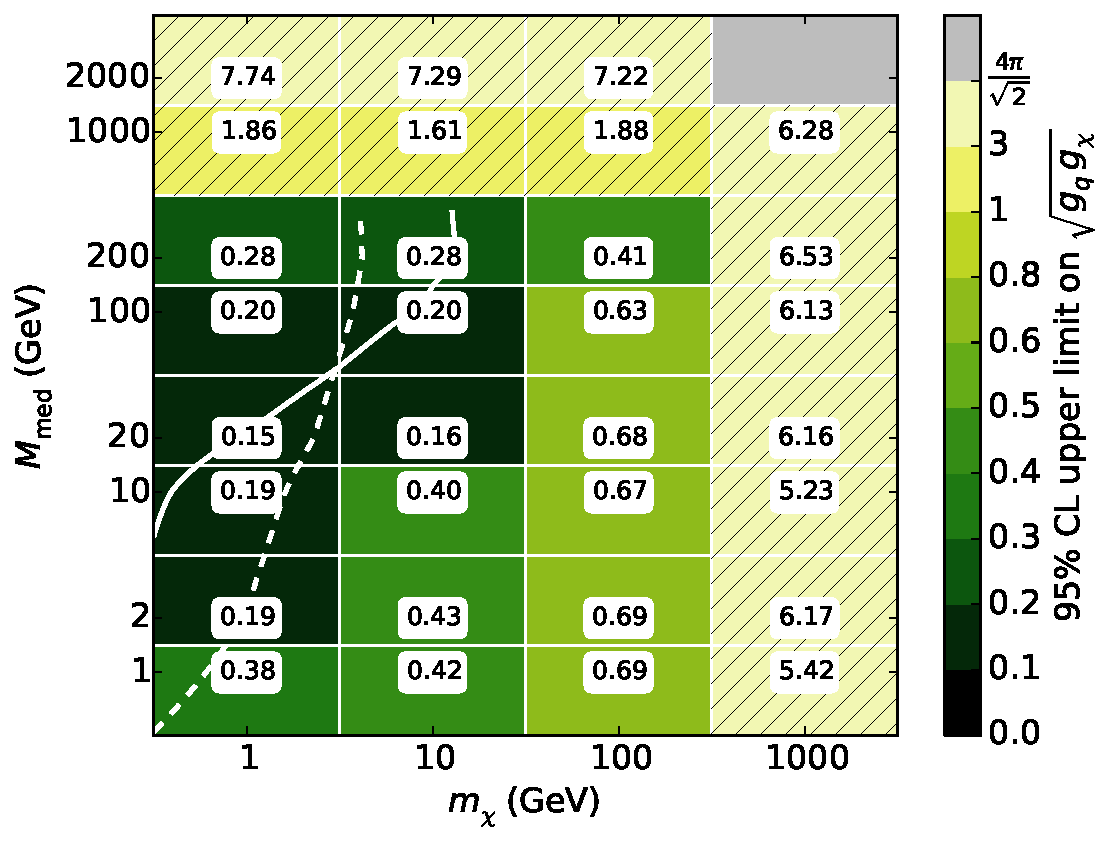
\includegraphics[width=1.\textwidth]{figures/grid_basepoints_SVD_rat05_monojet.pdf}
%    \caption{sV model, $g_q/g_{\chi} = 0.5$, \monojet channel.}
%  \end{subfigure}
%  \caption{}
%\end{figure}

\begin{sidewaysfigure}
  \centering
  \begin{subfigure}[t]{0.32\textwidth}
    \centering
    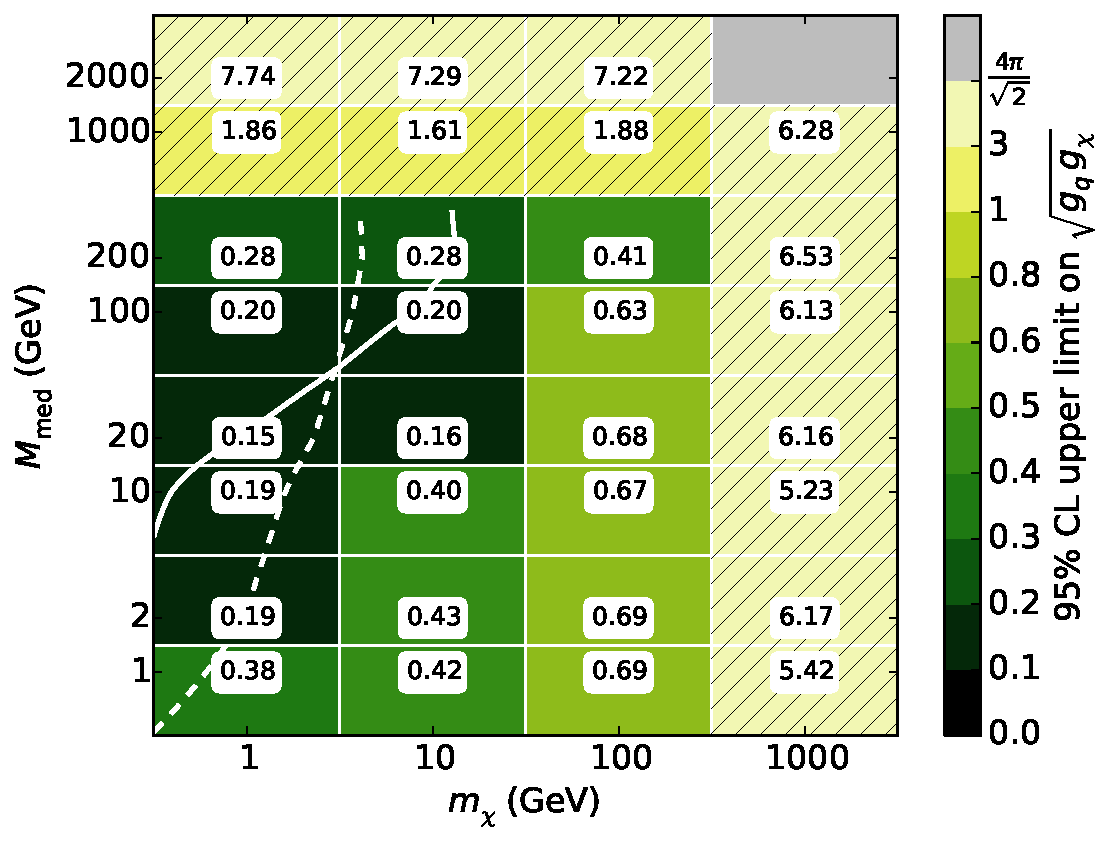
\includegraphics[width=1.\textwidth]{figures/grid_basepoints_SVD_rat05_monojet.pdf}
    \caption{$sV$ model, $\gX/\gq = 0.5$, \monojet channel.}
  \end{subfigure}
  \begin{subfigure}[t]{0.32\textwidth}
    \centering
    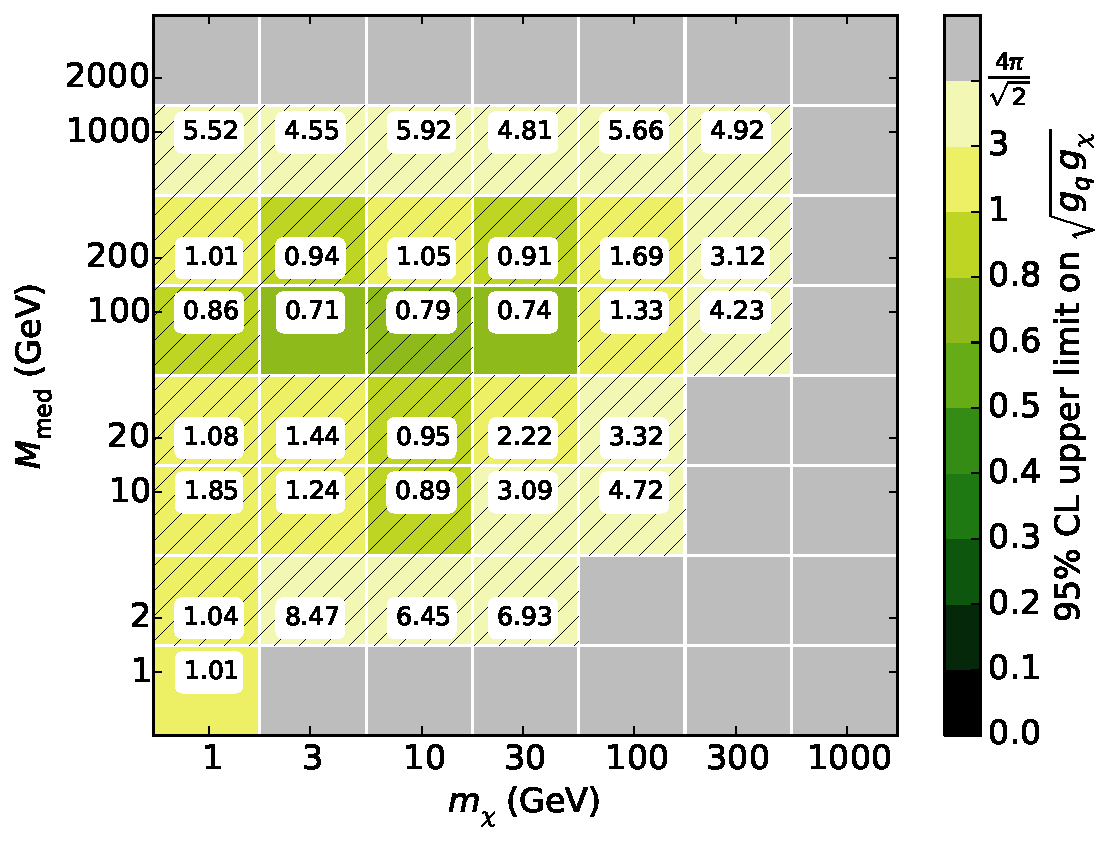
\includegraphics[width=1.\textwidth]{figures/grid_allpoints_SVD_rat05.pdf}
    \caption{$sV$ model, $\gX/\gq = 0.5$, mono-$Z$ channel.}
  \end{subfigure}
  \begin{subfigure}[t]{0.32\textwidth}
    \centering
    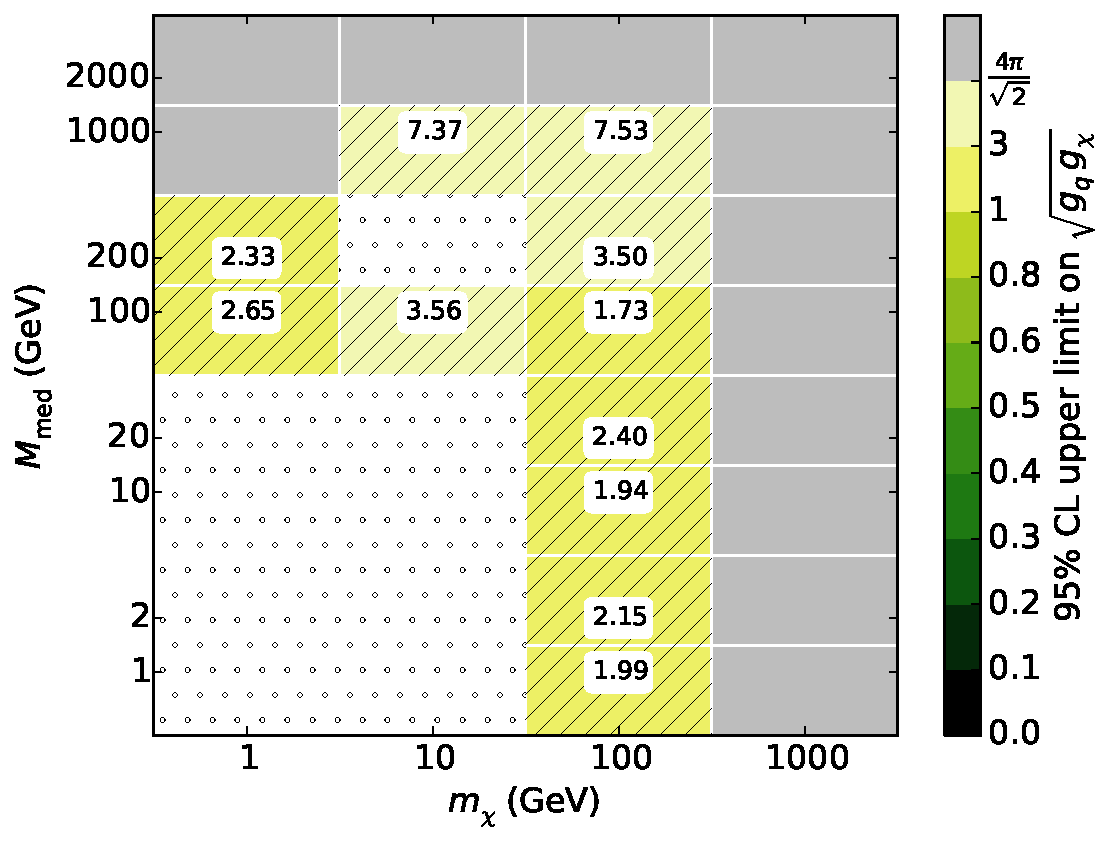
\includegraphics[width=1.\textwidth]{figures/grid_basepoints_SVD_rat05_monoWZ.pdf}
    \caption{$sV$ model, $\gX/\gq = 0.5$, mono-$W/Z$ channel.}
    \vspace{0.75cm}
  \end{subfigure}
  \begin{subfigure}[t]{0.32\textwidth}
    \centering
    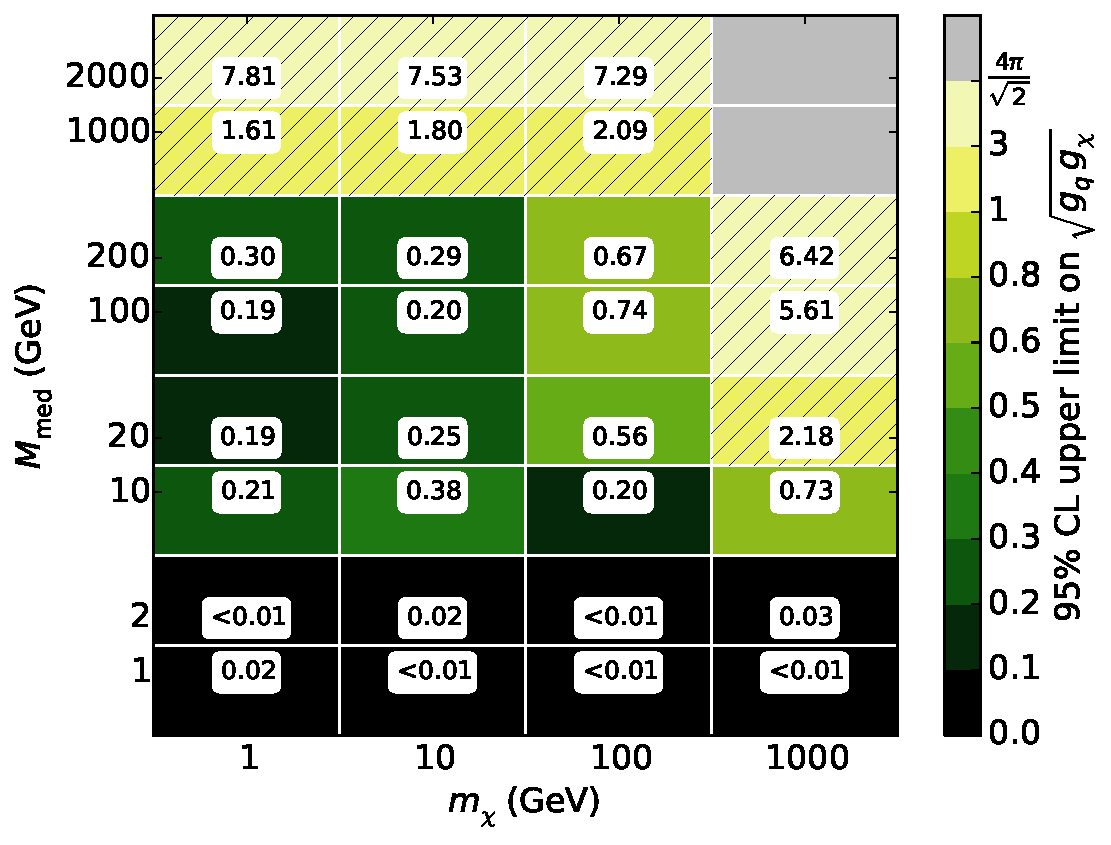
\includegraphics[width=1.\textwidth]{figures/grid_basepoints_SAD_rat05_monojet.pdf}
    \caption{$sA$ model, $\gX/\gq = 0.5$, \monojet channel.}
  \end{subfigure}
  \begin{subfigure}[t]{0.32\textwidth}
    \centering
    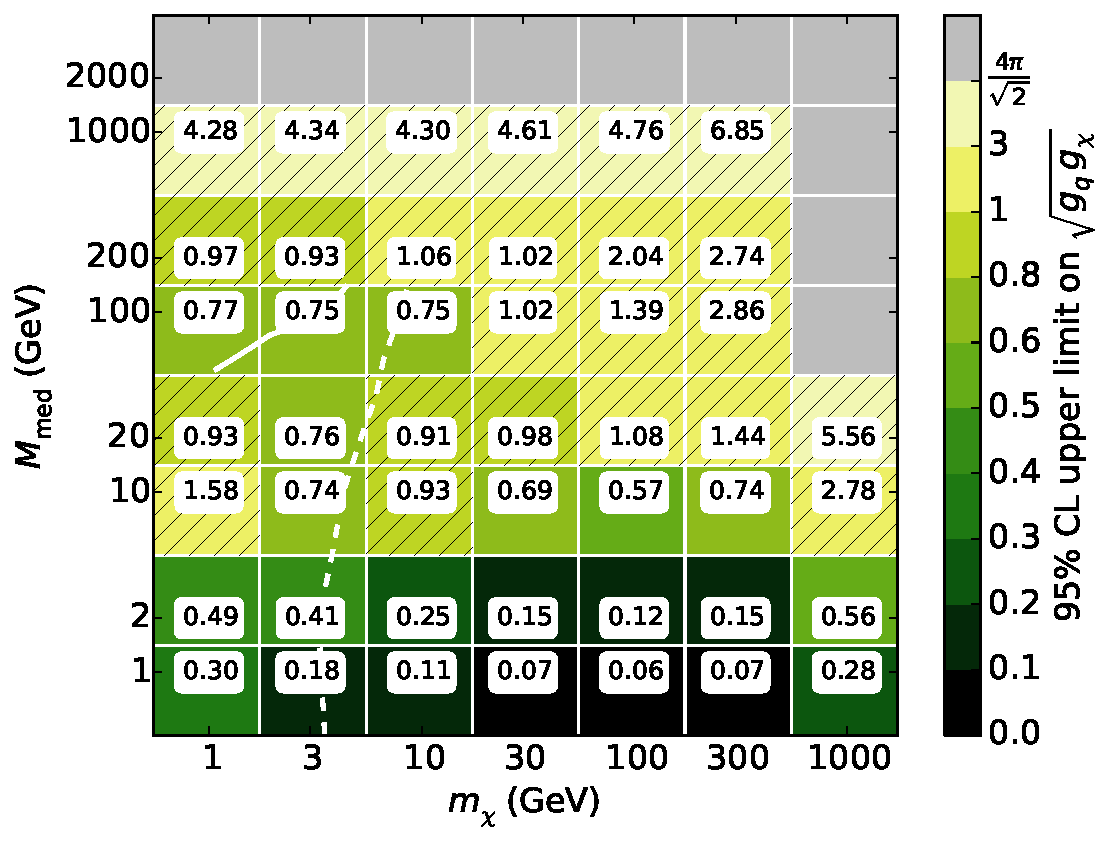
\includegraphics[width=1.\textwidth]{figures/grid_allpoints_SAD_rat05.pdf}
    \caption{$sA$ model, $\gX/\gq = 0.5$, mono-$Z$ channel.}
  \end{subfigure}
  \begin{subfigure}[t]{0.32\textwidth}
    \centering
    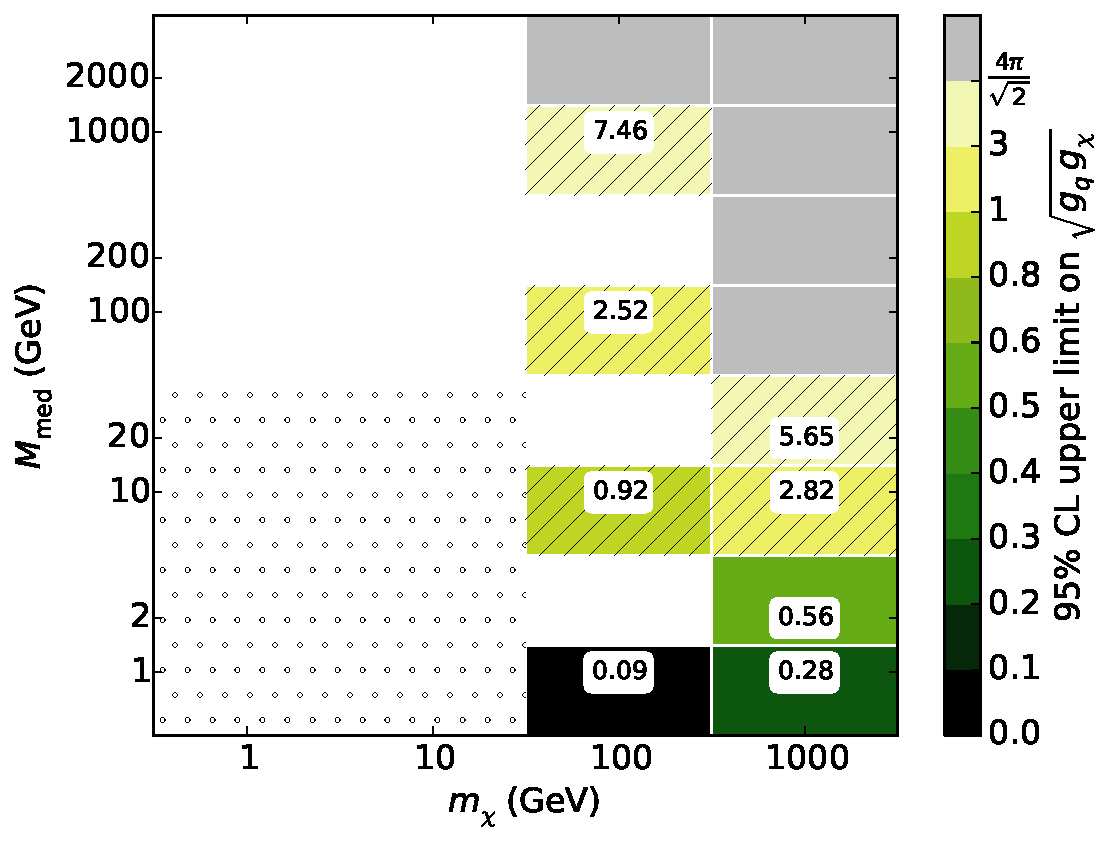
\includegraphics[width=1.\textwidth]{figures/grid_basepoints_SAD_rat05_monoWZ.pdf}
    \caption{$sA$ model, $\gX/\gq = 0.5$, mono-$W/Z$ channel.}
  \end{subfigure}
  \caption{Upper limits on the coupling for the $s$-channel models in the \monojet (left), \monoZ (centre) and \monoWZ (right) channels, for $\gX / \gq$ = 0.5. The grey region represents the phase space where no meaningful limit was obtained. The hatched region represents a limit which leads to a width greater than $\Mmed / 2$, so the validity of the calculation begins to fail. The dotted region represents phase space where insufficient statistics were available.}
  \label{fig:results_sVsA_rat05}
\end{sidewaysfigure}

\begin{sidewaysfigure}
  \centering
  \begin{subfigure}[t]{0.32\textwidth}
    \centering
    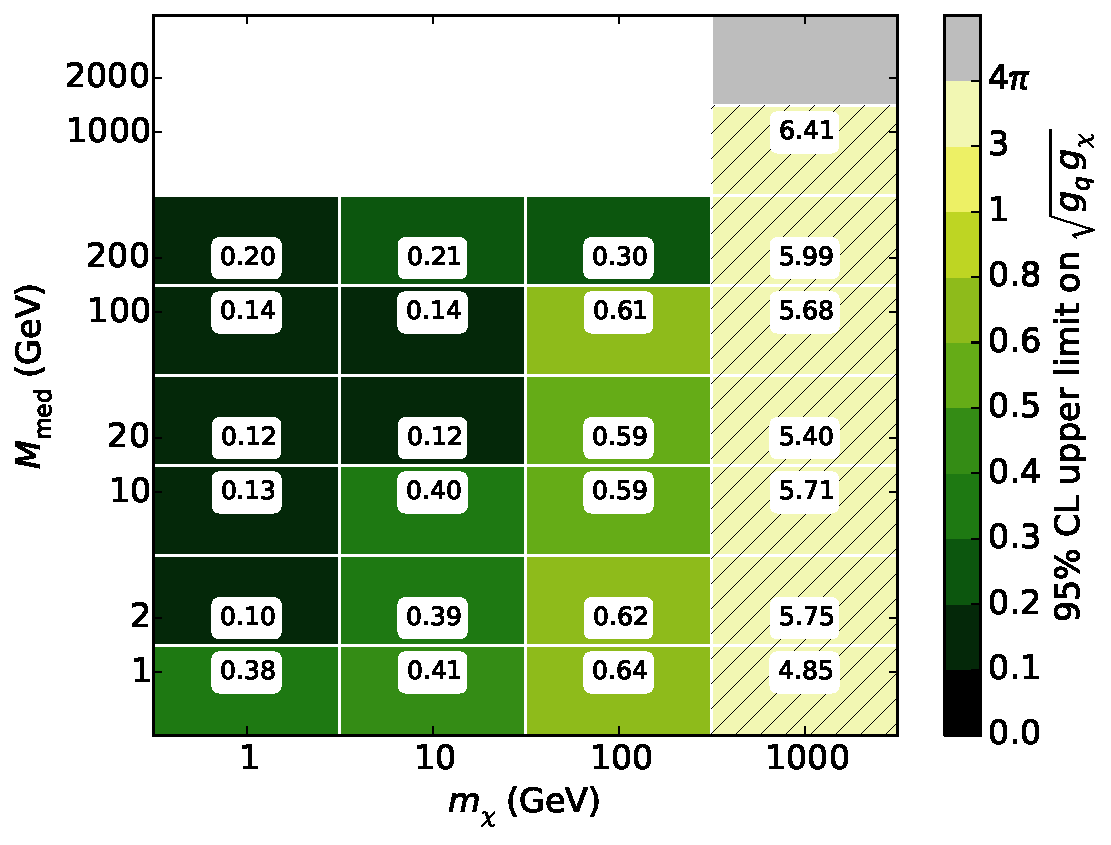
\includegraphics[width=1.\textwidth]{figures/grid_basepoints_SVD_rat1_monojet.pdf}
    \caption{$sV$ model, $\gX/\gq = 1$, \monojet channel.}
  \end{subfigure}
  \begin{subfigure}[t]{0.32\textwidth}
    \centering
    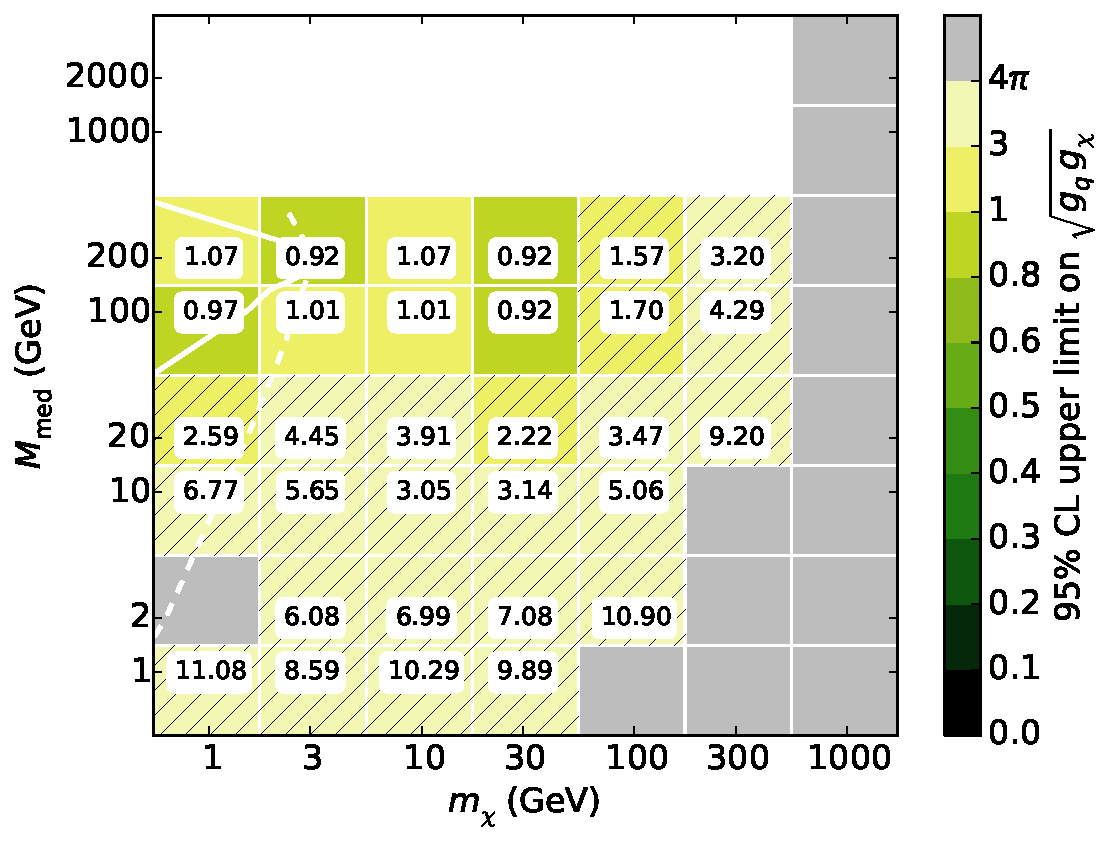
\includegraphics[width=1.\textwidth]{figures/grid_allpoints_SVD_rat1.pdf}
    \caption{$sV$ model, $\gX/\gq = 1$, mono-$Z$ channel.}
  \end{subfigure}
  \begin{subfigure}[t]{0.32\textwidth}
    \centering
    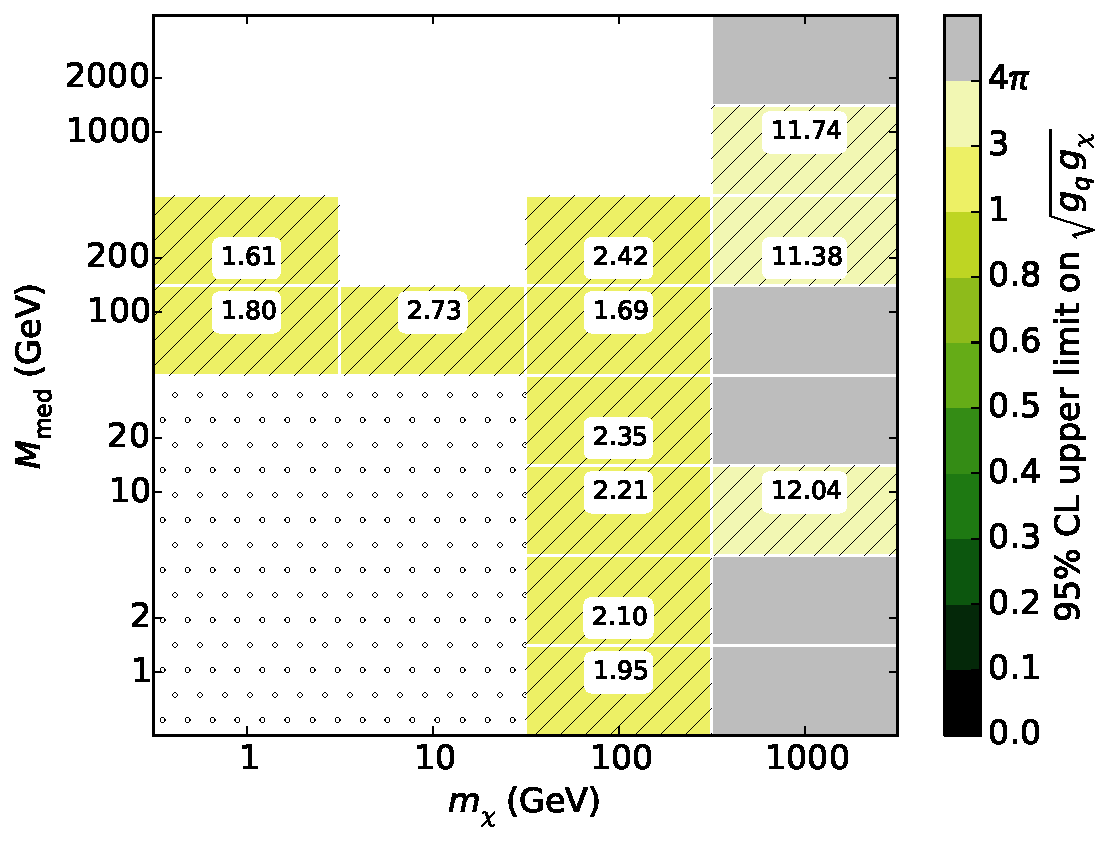
\includegraphics[width=1.\textwidth]{figures/grid_basepoints_SVD_rat1_monoWZ.pdf}
    \caption{$sV$ model, $\gX/\gq = 1$, mono-$W/Z$ channel.}
    \vspace{0.75cm}
  \end{subfigure}
  \begin{subfigure}[t]{0.32\textwidth}
    \centering
    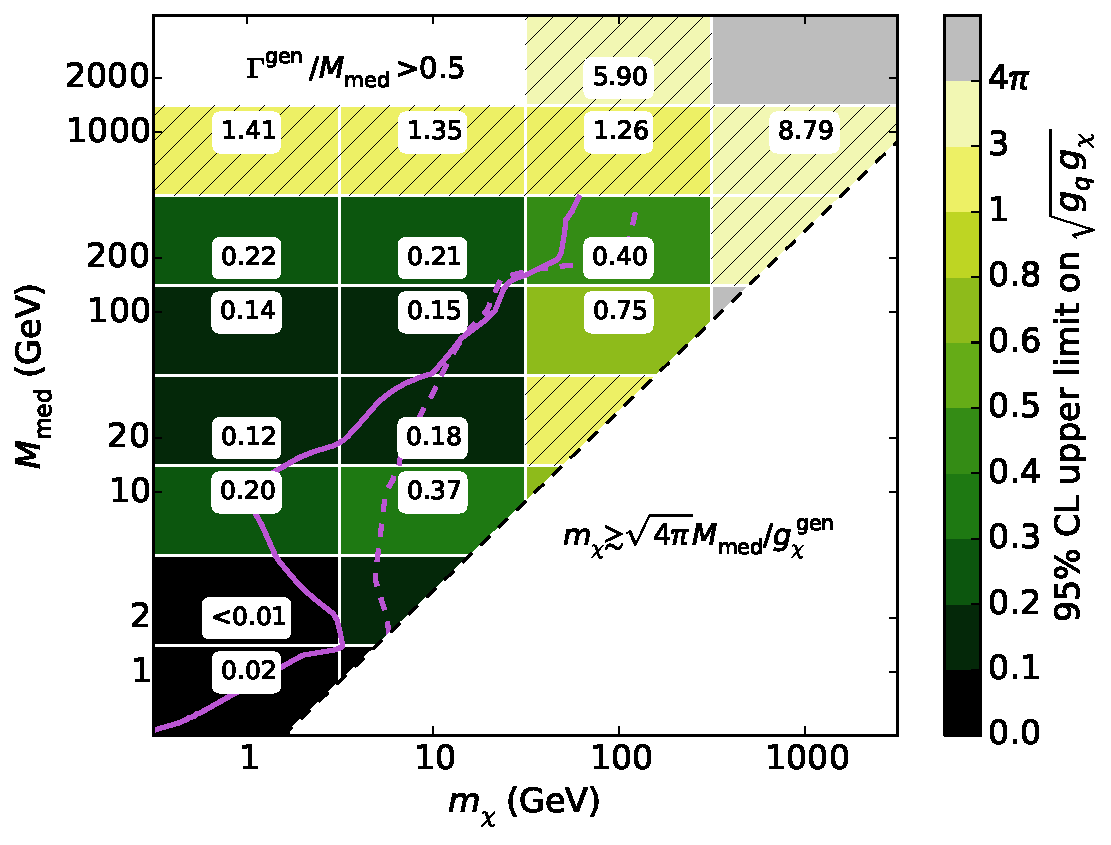
\includegraphics[width=1.\textwidth]{figures/grid_basepoints_SAD_rat1_monojet.pdf}
    \caption{$sA$ model, $\gX/\gq = 1$, \monojet channel.}
  \end{subfigure}
  \begin{subfigure}[t]{0.32\textwidth}
    \centering
    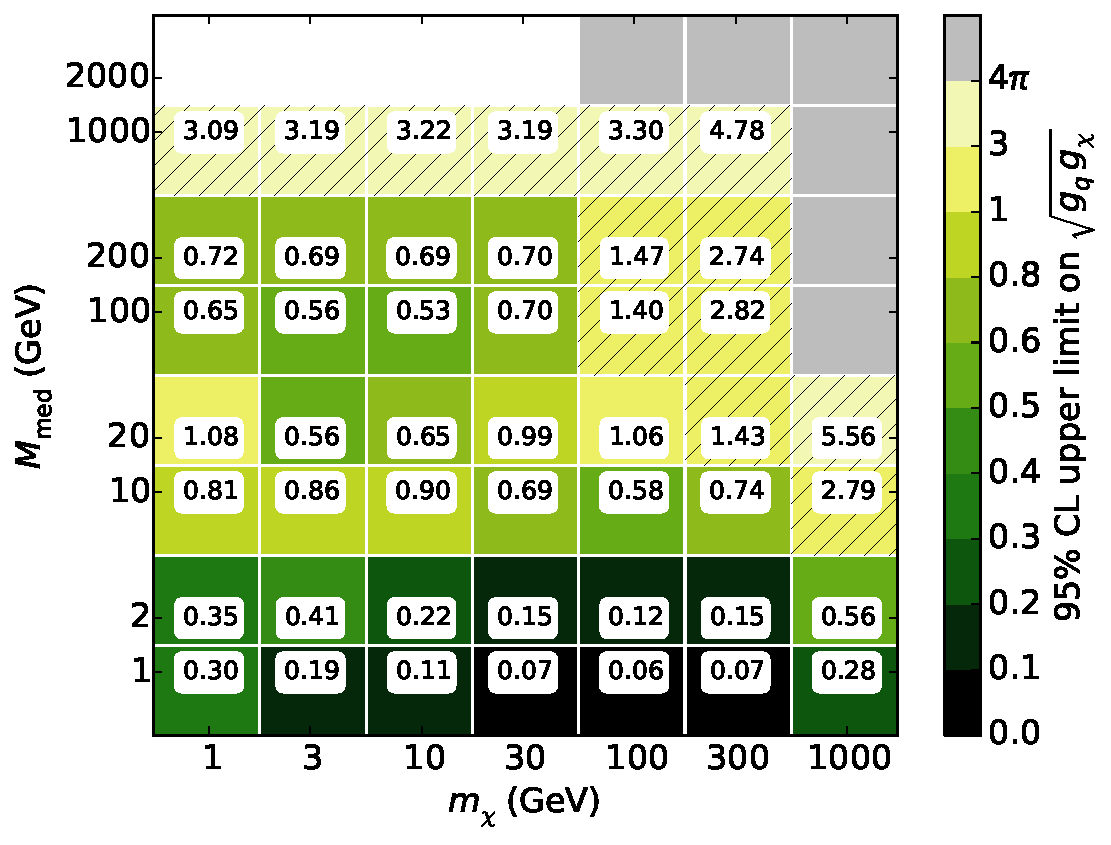
\includegraphics[width=1.\textwidth]{figures/grid_allpoints_SAD_rat1.pdf}
    \caption{$sA$ model, $\gX/\gq = 1$, mono-$Z$ channel.}
  \end{subfigure}
  \begin{subfigure}[t]{0.32\textwidth}
    \centering
    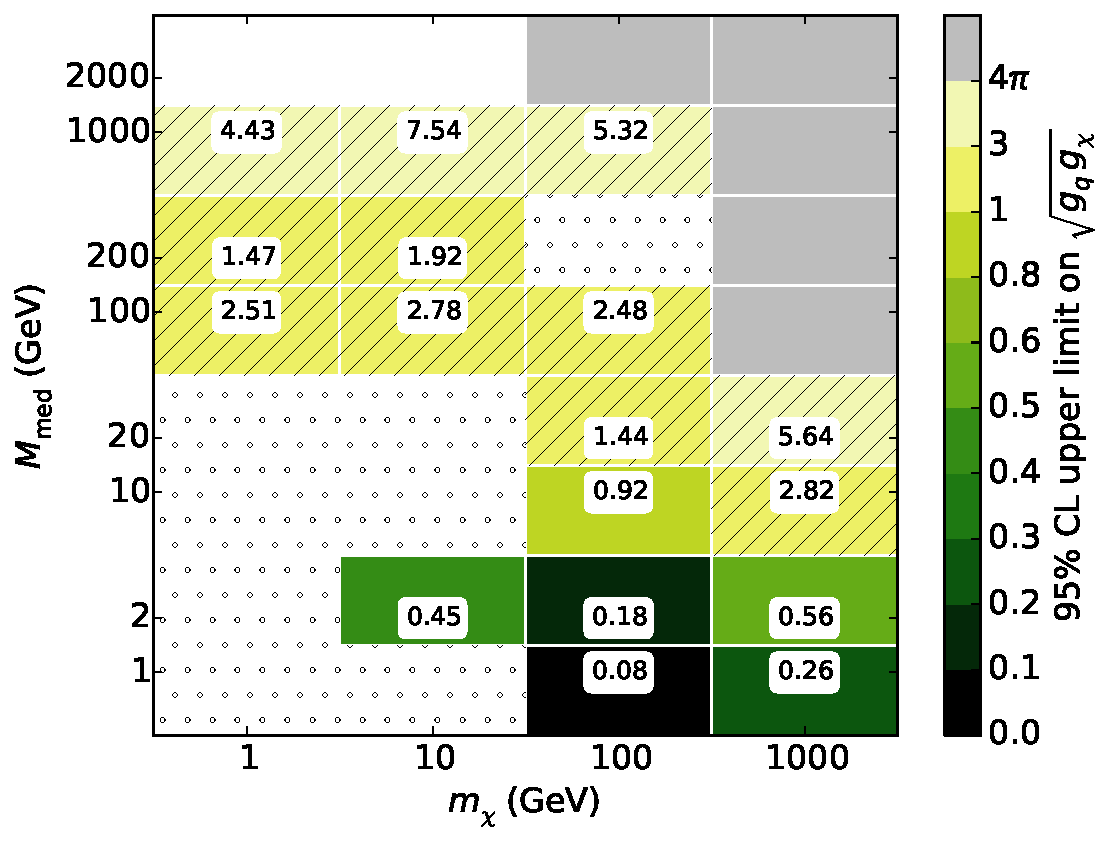
\includegraphics[width=1.\textwidth]{figures/grid_basepoints_SAD_rat1_monoWZ.pdf}
    \caption{$sA$ model, $\gX/\gq = 1$, mono-$W/Z$ channel.}
  \end{subfigure}
  \caption{Upper limits on the couplings for the $s$-channel models in the \monojet (left), \monoZ (centre) and \monoWZ (right) channels, for $\gX / \gq$ = 1. Refer to fig.~\ref{fig:results_sVsA_rat05} for details.}
  \label{fig:results_sVsA_rat1}
\end{sidewaysfigure}

\begin{sidewaysfigure}
  \centering
  \begin{subfigure}[t]{0.32\textwidth}
    \centering
    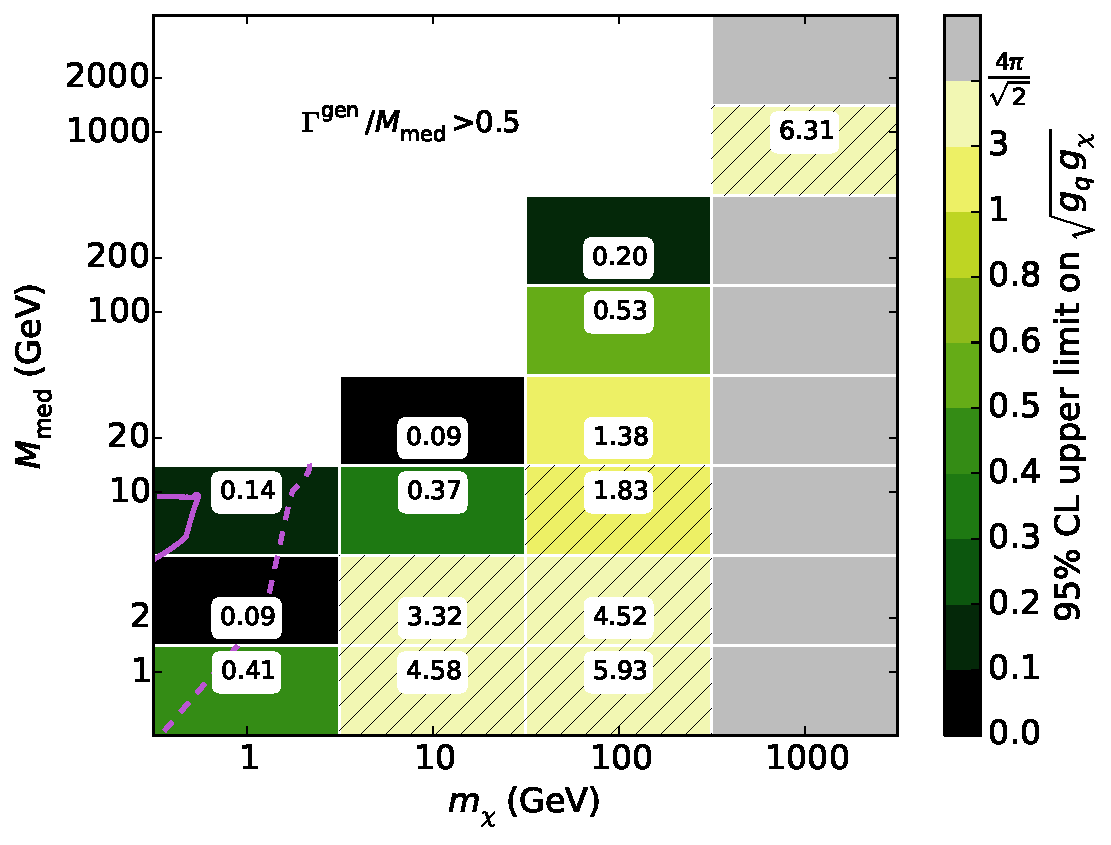
\includegraphics[width=1.\textwidth]{figures/grid_basepoints_SVD_rat2_monojet.pdf}
    \caption{$sV$ model, $\gX/\gq = 2$, \monojet channel.}
  \end{subfigure}
  \begin{subfigure}[t]{0.32\textwidth}
    \centering
    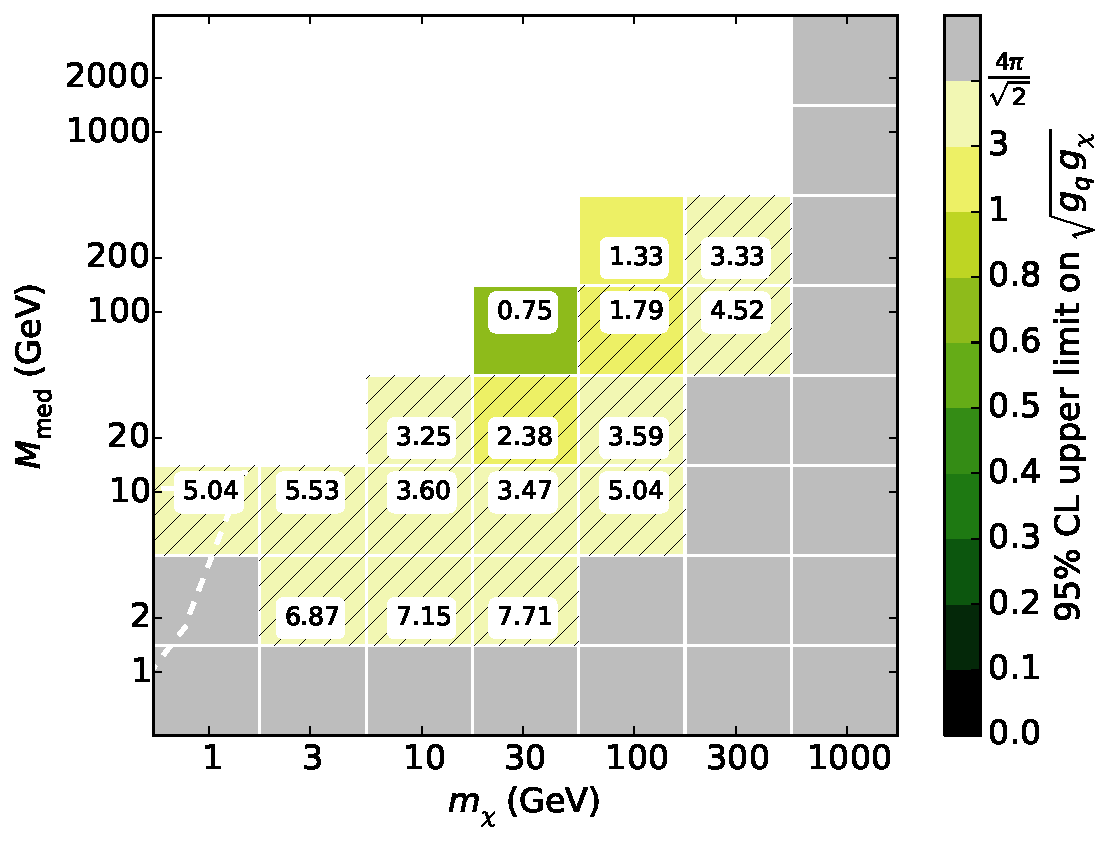
\includegraphics[width=1.\textwidth]{figures/grid_allpoints_SVD_rat2.pdf}
    \caption{$sV$ model, $\gX/\gq = 2$, mono-$Z$ channel.}
  \end{subfigure}
  \begin{subfigure}[t]{0.32\textwidth}
    \centering
    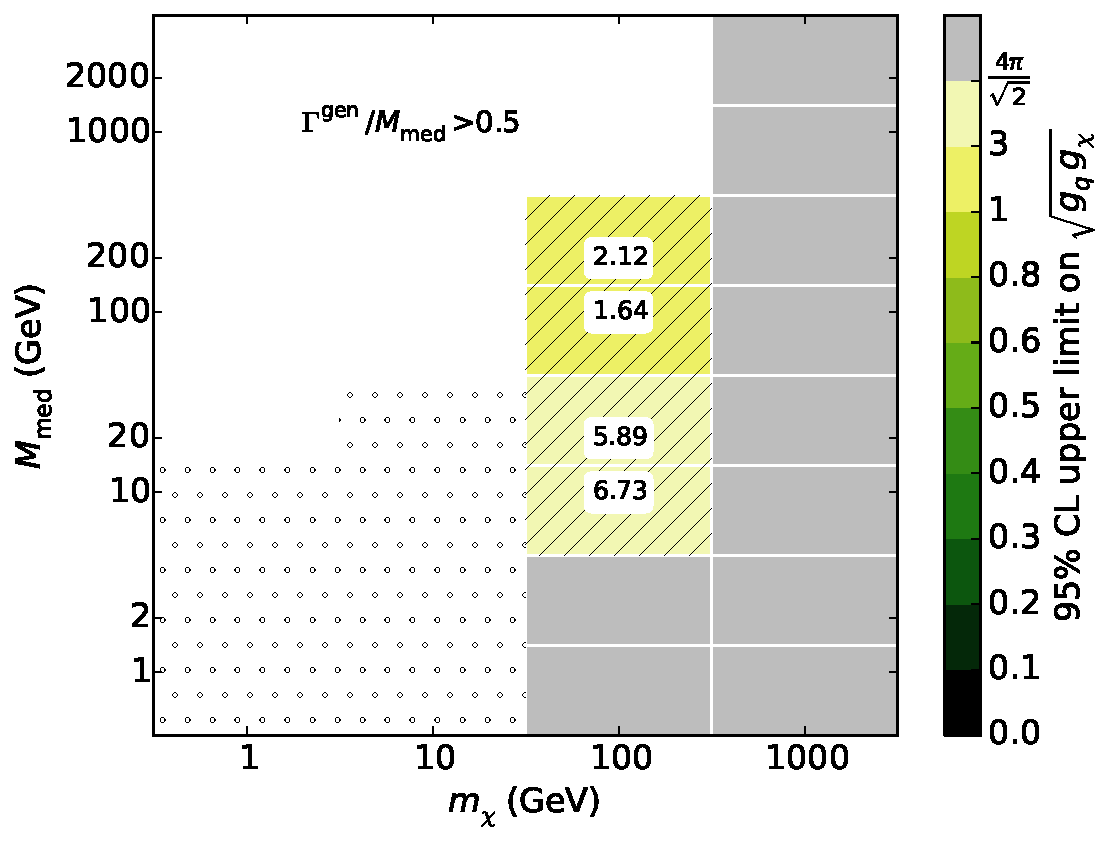
\includegraphics[width=1.\textwidth]{figures/grid_basepoints_SVD_rat2_monoWZ.pdf}
    \caption{$sV$ model, $\gX/\gq = 2$, mono-$W/Z$ channel.}
    \vspace{0.75cm}
  \end{subfigure}
  \begin{subfigure}[t]{0.32\textwidth}
    \centering
    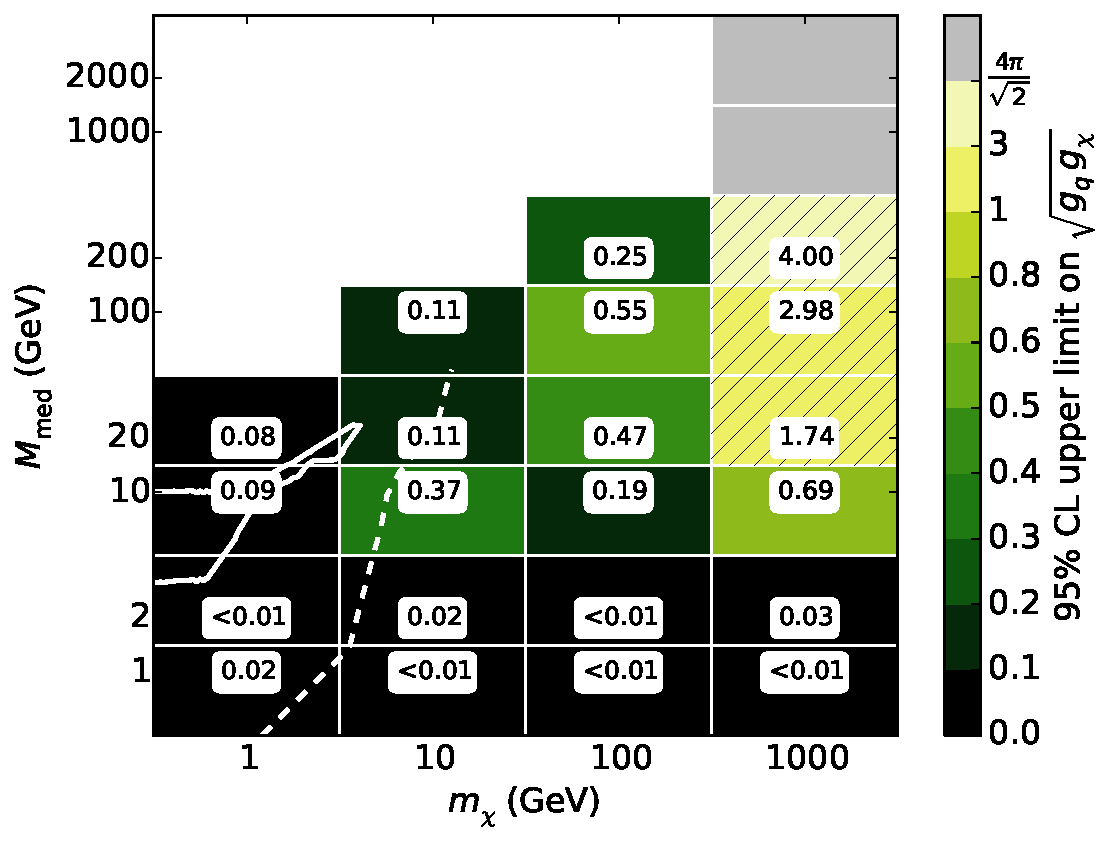
\includegraphics[width=1.\textwidth]{figures/grid_basepoints_SAD_rat2_monojet.pdf}
    \caption{$sA$ model, $\gX/\gq = 2$, \monojet channel.}
  \end{subfigure}
  \begin{subfigure}[t]{0.32\textwidth}
    \centering
    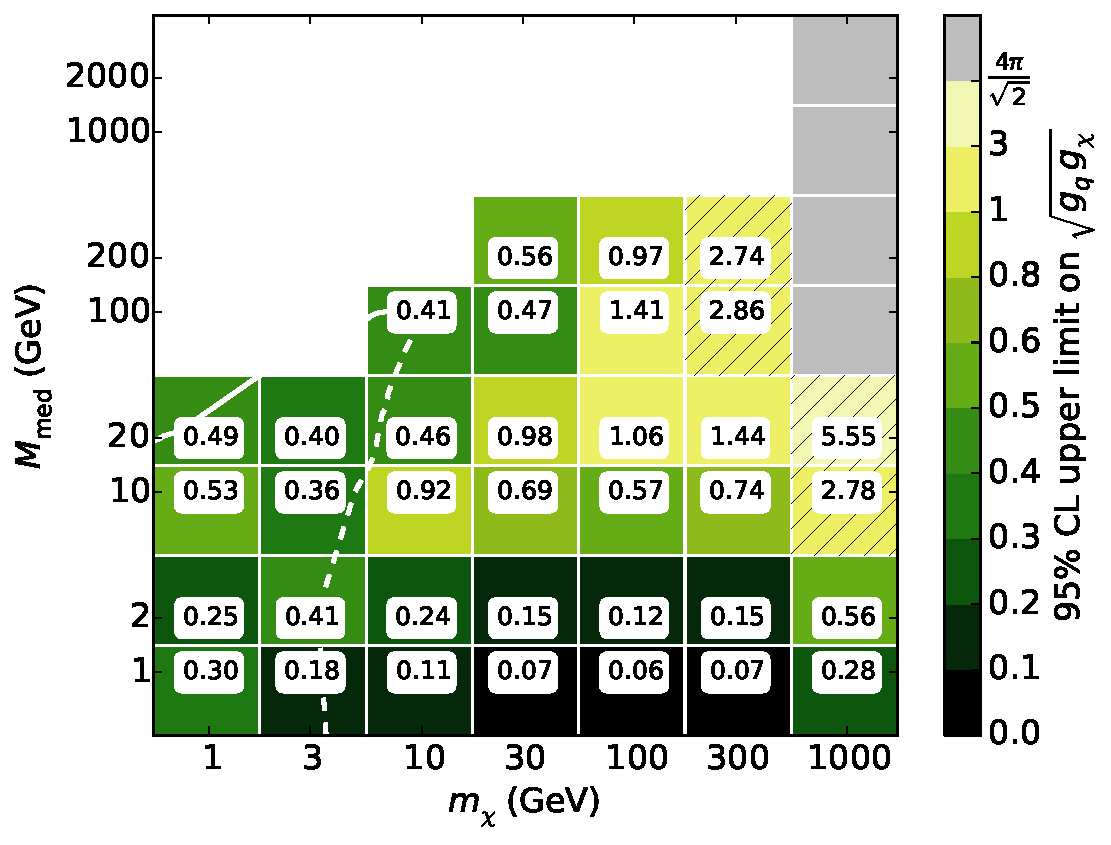
\includegraphics[width=1.\textwidth]{figures/grid_allpoints_SAD_rat2.pdf}
    \caption{$sA$ model, $\gX/\gq = 2$, mono-$Z$ channel.}
  \end{subfigure}
  \begin{subfigure}[t]{0.32\textwidth}
    \centering
    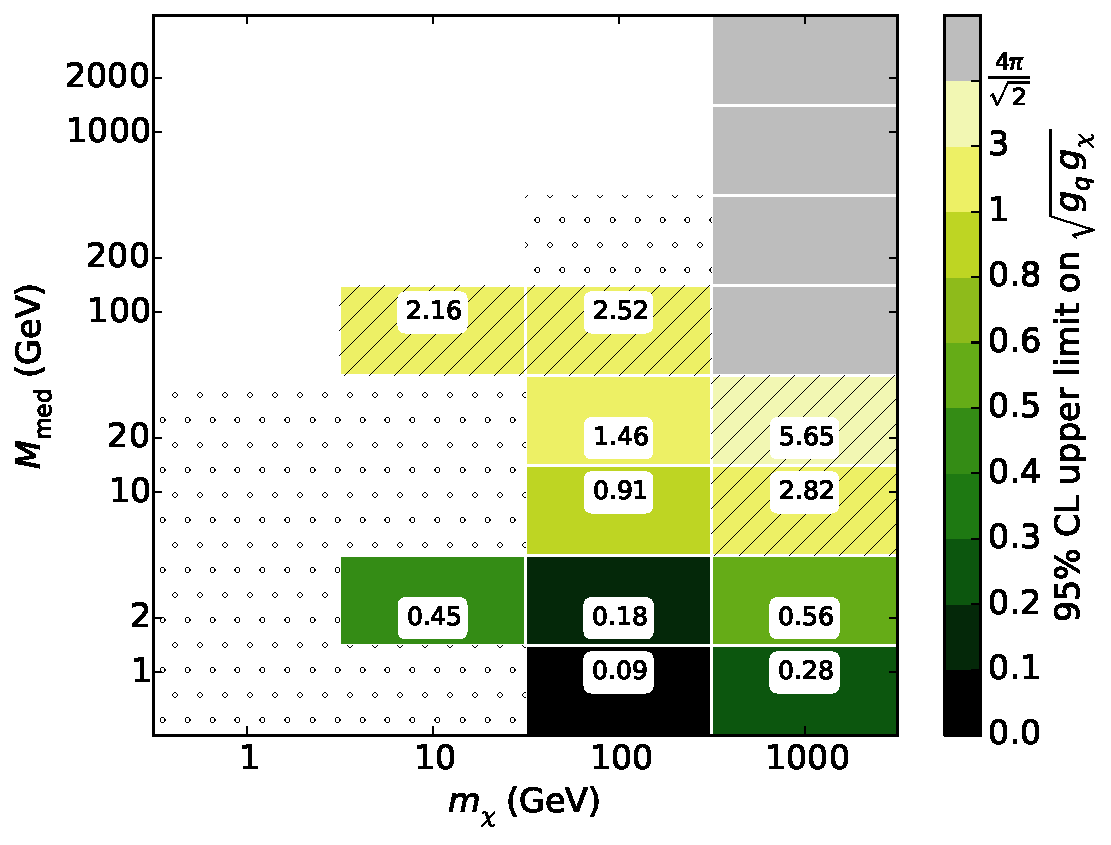
\includegraphics[width=1.\textwidth]{figures/grid_basepoints_SAD_rat2_monoWZ.pdf}
    \caption{$sA$ model, $\gX/\gq = 2$, mono-$W/Z$ channel.}
  \end{subfigure}
  \caption{Upper limits on the coupling for the $s$-channel models in the \monojet (left), \monoZ (centre) and \monoWZ (right) channels, for $\gX / \gq$ = 2. Refer to fig.~\ref{fig:results_sVsA_rat05} for details.}
  \label{fig:results_sVsA_rat2}
\end{sidewaysfigure}

\begin{sidewaysfigure}
  \centering
  \begin{subfigure}[t]{0.32\textwidth}
    \centering
    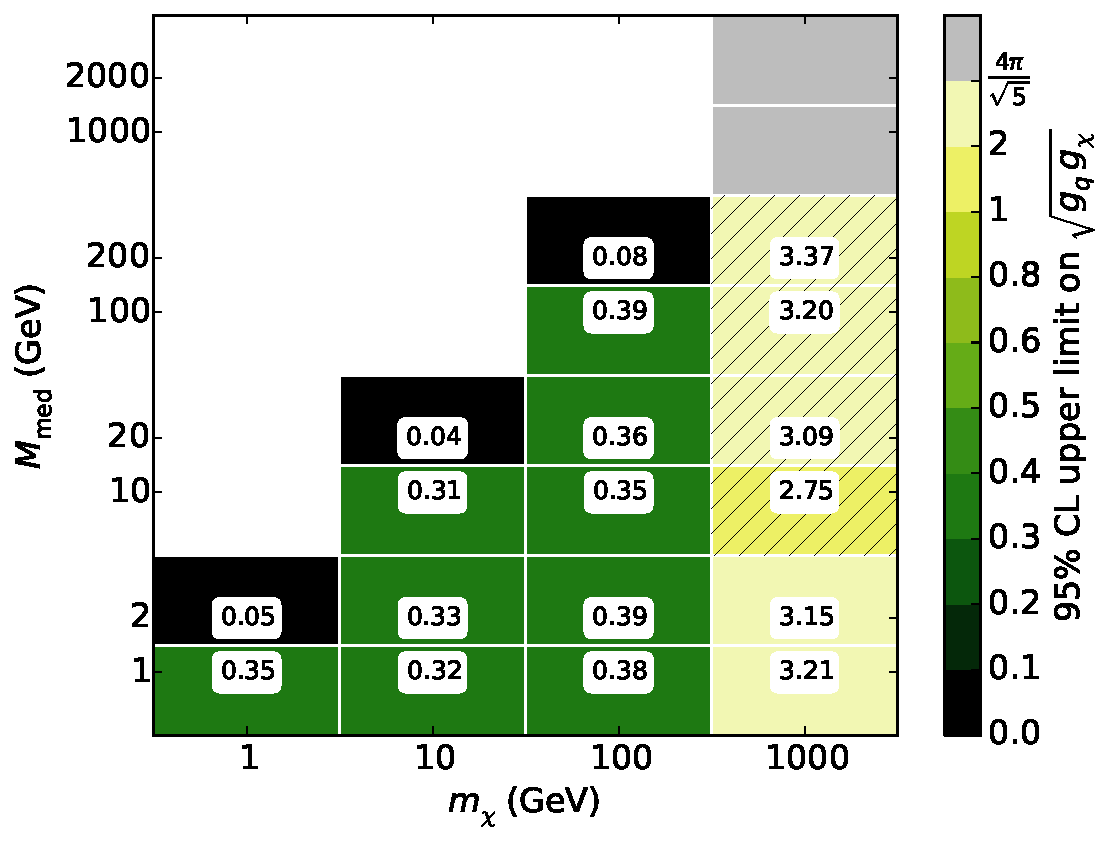
\includegraphics[width=1.\textwidth]{figures/grid_basepoints_SVD_rat5_monojet.pdf}
    \caption{$sV$ model, $\gX/\gq = 5$, \monojet channel.}
  \end{subfigure}
  \begin{subfigure}[t]{0.32\textwidth}
    \centering
    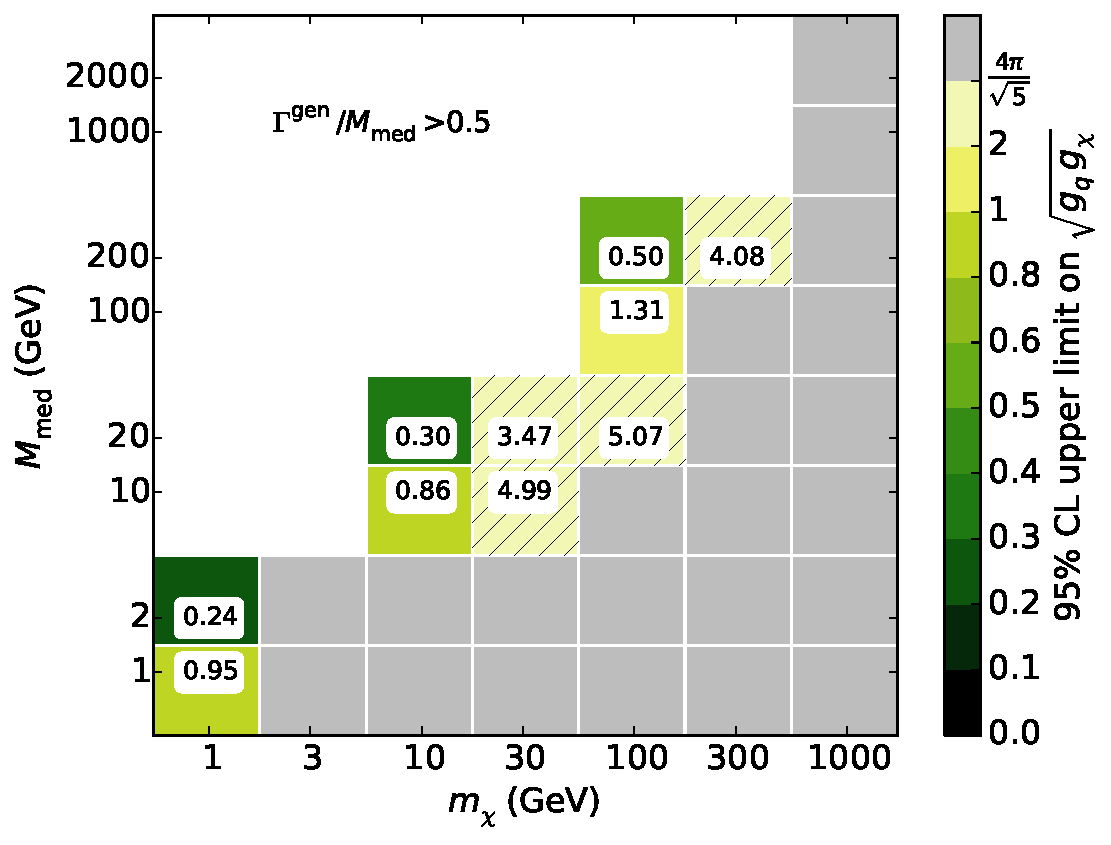
\includegraphics[width=1.\textwidth]{figures/grid_allpoints_SVD_rat5.pdf}
    \caption{$sV$ model, $\gX/\gq = 5$, mono-$Z$ channel.}
  \end{subfigure}
  \begin{subfigure}[t]{0.32\textwidth}
    \centering
    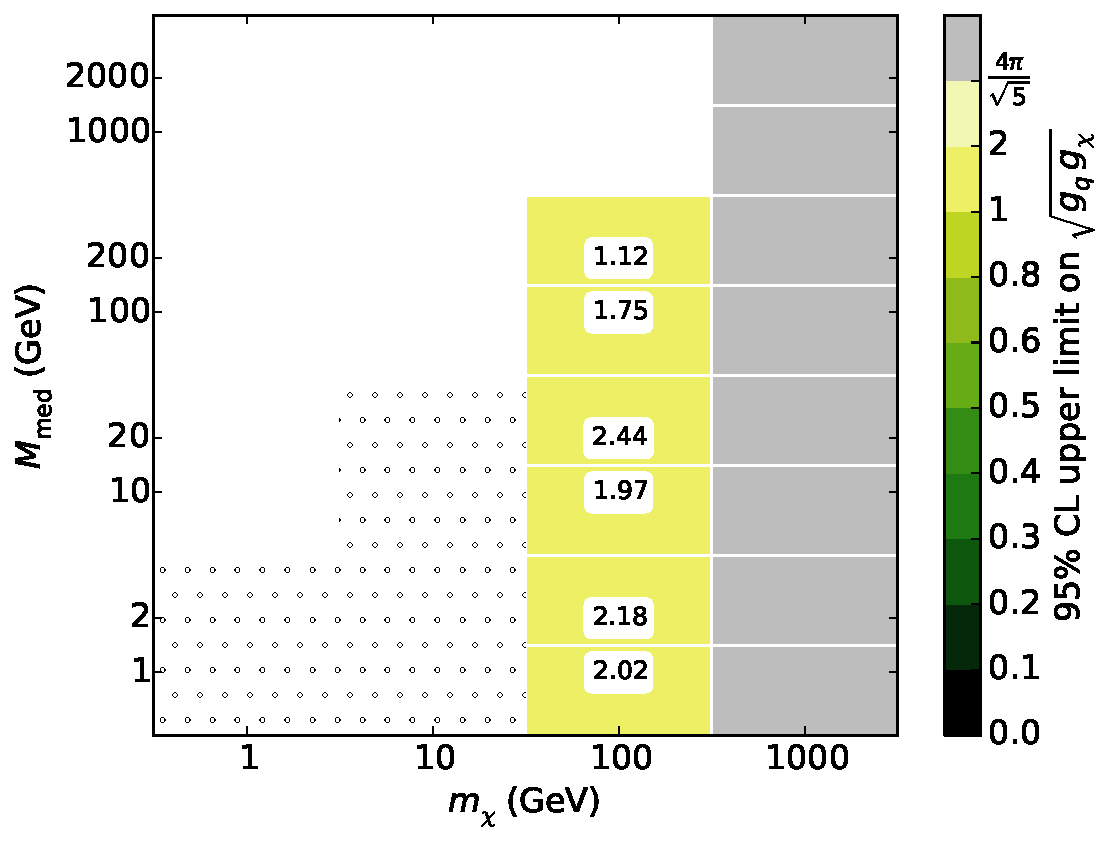
\includegraphics[width=1.\textwidth]{figures/grid_basepoints_SVD_rat5_monoWZ.pdf}
    \caption{$sV$ model, $\gX/\gq = 5$, mono-$W/Z$ channel.}
    \vspace{0.75cm}
  \end{subfigure}
  \begin{subfigure}[t]{0.32\textwidth}
    \centering
    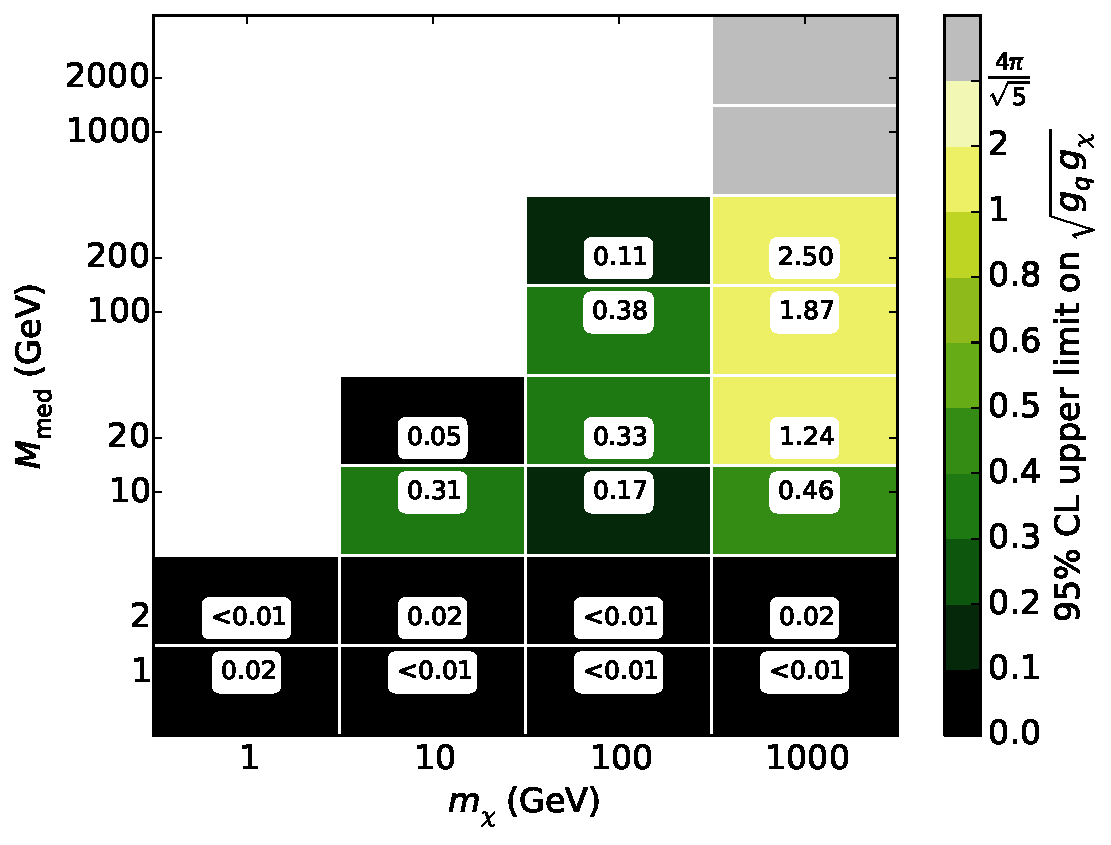
\includegraphics[width=1.\textwidth]{figures/grid_basepoints_SAD_rat5_monojet.pdf}
    \caption{$sA$ model, $\gX/\gq = 5$, \monojet channel.}
  \end{subfigure}
  \begin{subfigure}[t]{0.32\textwidth}
    \centering
    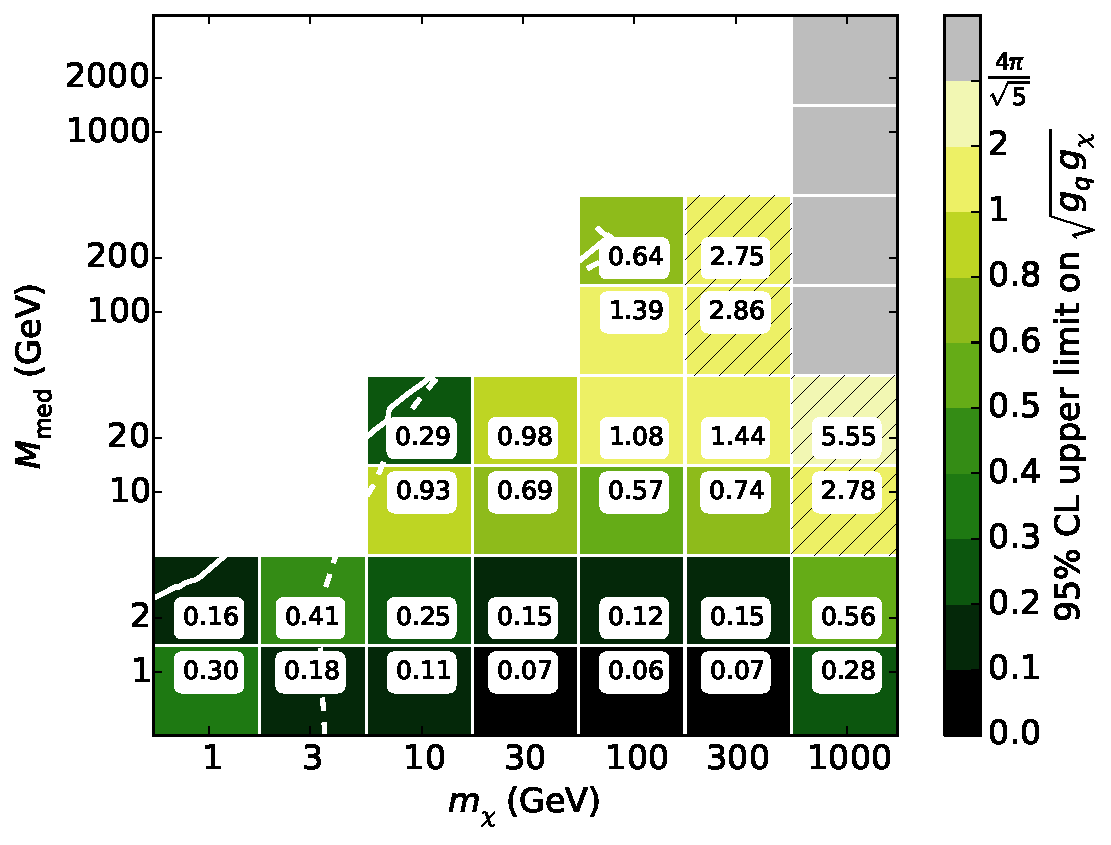
\includegraphics[width=1.\textwidth]{figures/grid_allpoints_SAD_rat5.pdf}
    \caption{$sA$ model, $\gX/\gq = 5$, mono-$Z$ channel.}
  \end{subfigure}
  \begin{subfigure}[t]{0.32\textwidth}
    \centering
    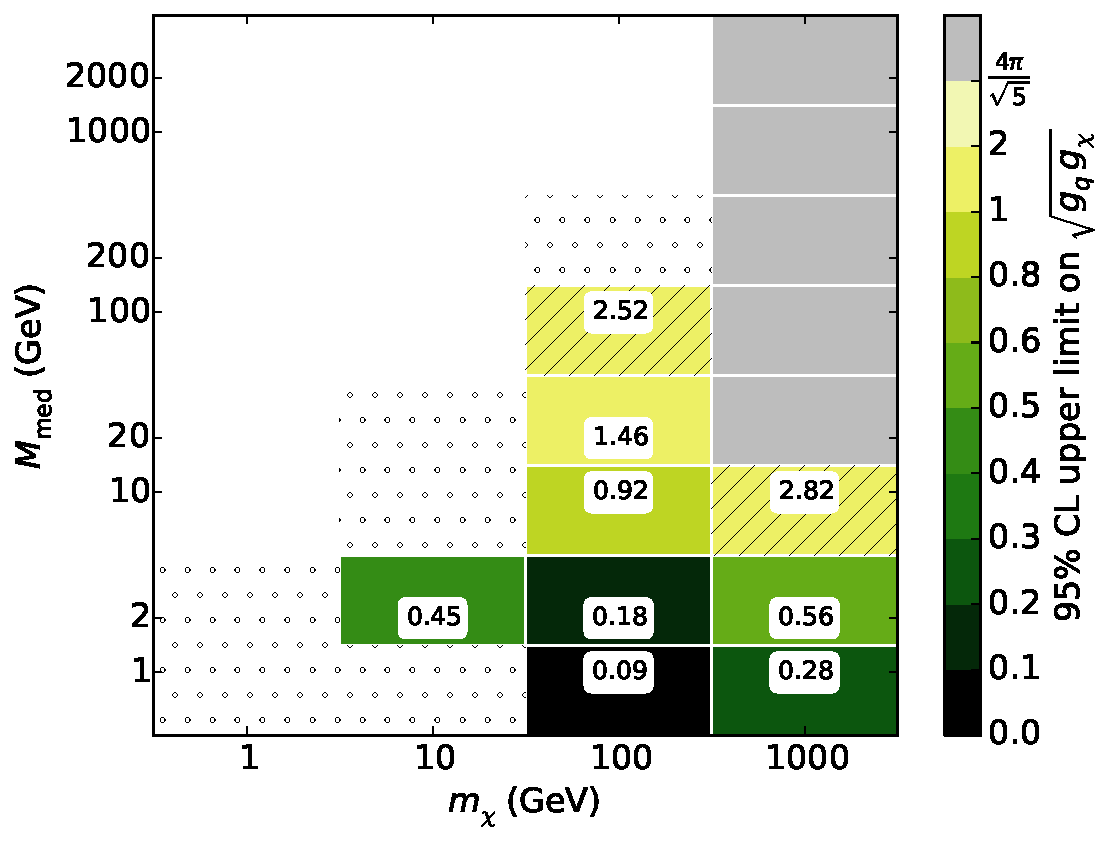
\includegraphics[width=1.\textwidth]{figures/grid_basepoints_SAD_rat5_monoWZ.pdf}
    \caption{$sA$ model, $\gX/\gq = 5$, mono-$W/Z$ channel.}
  \end{subfigure}
  \caption{Upper limits on the coupling for the $s$-channel models in the \monojet (left), \monoZ (centre) and \monoWZ (right) channels, for $\gX / \gq$ = 5. Refer to fig.~\ref{fig:results_sVsA_rat05} for details.}
  \label{fig:results_sVsA_rat5}
\end{sidewaysfigure}

\begin{figure}
  \centering
  \begin{subfigure}[t]{0.495\textwidth}
    \centering
    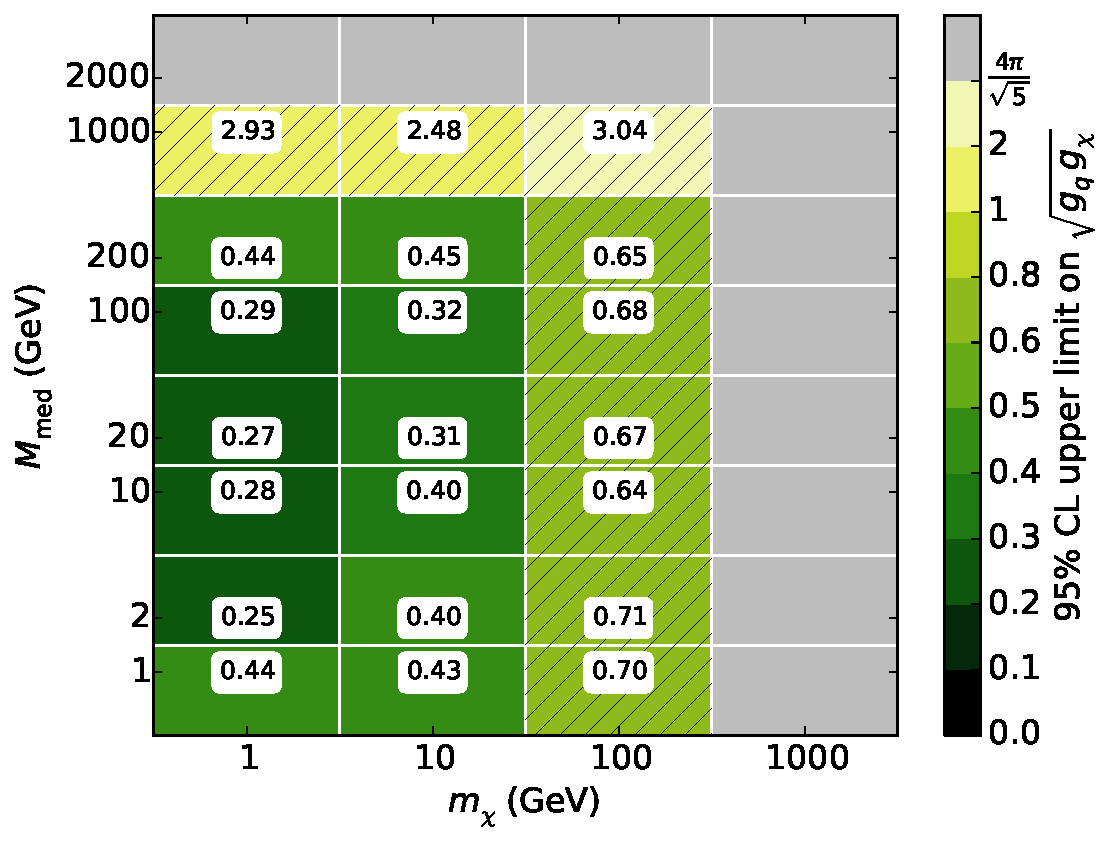
\includegraphics[width=1.\textwidth]{figures/grid_basepoints_SVD_rat02_monojet.pdf}
    \caption{$sV$ model, $\gX/\gq = 0.2$, \monojet channel.}
  \end{subfigure}
  \begin{subfigure}[t]{0.495\textwidth}
    \centering
    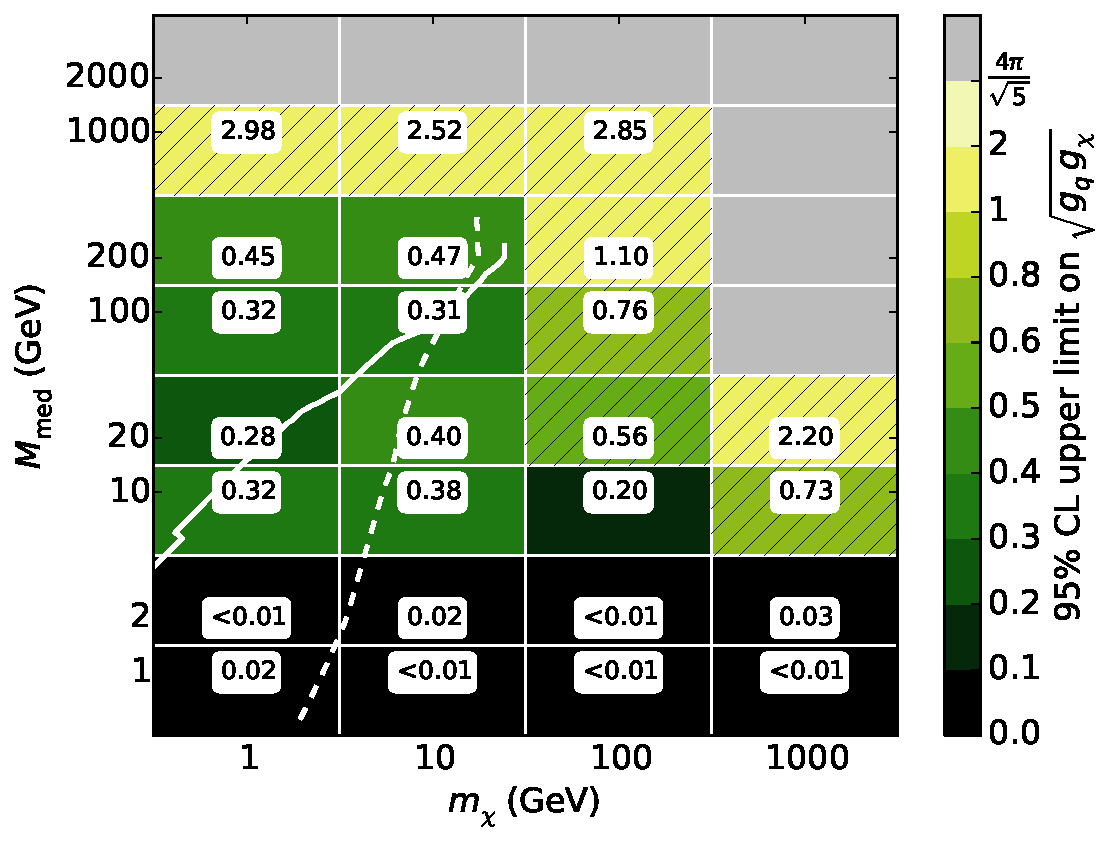
\includegraphics[width=1.\textwidth]{figures/grid_basepoints_SAD_rat02_monojet.pdf}
    \caption{$sA$ model, $\gX/\gq = 0.2$, \monojet channel.}
  \end{subfigure}
  \caption{Upper limits on the coupling for the $s$-channel models in the \monojet channel, for $\gX / \gq$ = 0.2. Refer to fig.~\ref{fig:results_sVsA_rat05} for details.}
  \label{fig:results_sVsA_rat02}
\end{figure}

\begin{figure}
  \centering
  \begin{subfigure}[t]{0.495\textwidth}
    \centering
    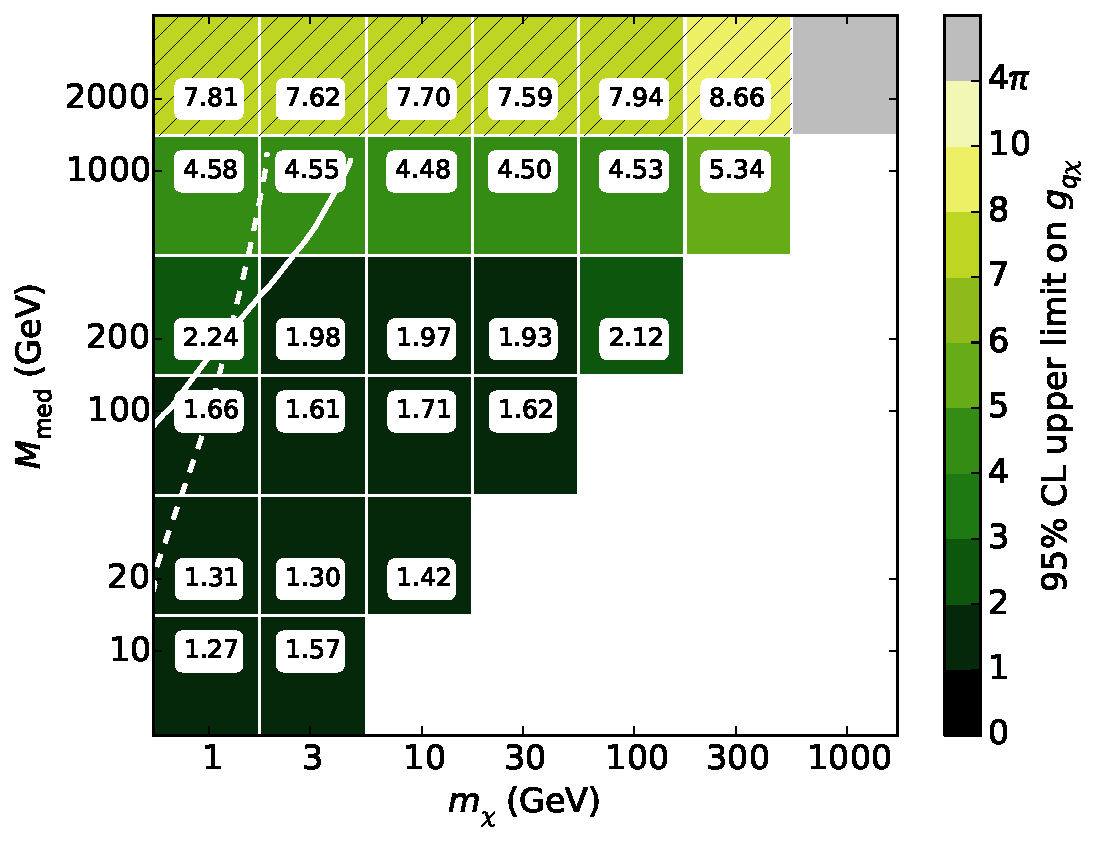
\includegraphics[width=1.\textwidth]{figures/grid_allpoints_TSD_rat1.pdf}
    \caption{$tS$ model, mono-$Z$ channel.}
  \end{subfigure}
  \begin{subfigure}[t]{0.495\textwidth}
    \centering
    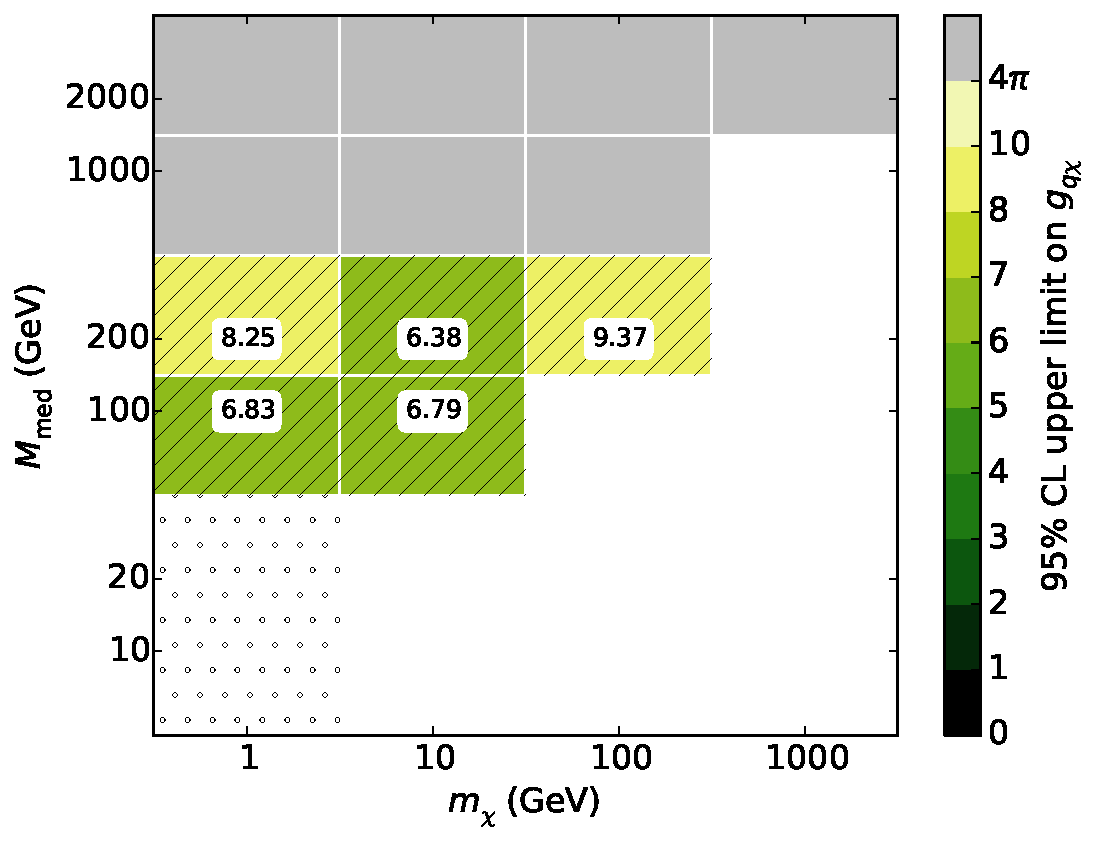
\includegraphics[width=1.\textwidth]{figures/grid_basepoints_TSD_rat1_monoWZ.pdf}
    \caption{$tS$ model, mono-$W/Z$ channel.}
  \end{subfigure}
  \caption{Upper limits on the coupling $\gqX$ for the $t$-channel model in the \monoZ (left) and \monoWZ (right) channels. Refer to fig.~\ref{fig:results_sVsA_rat05} for details.}
  \label{fig:results_tS}
\end{figure}

\subsection{Comparison with Relic Density Constraints}
%%%%%%%%%%%%%%%%%%%%%%%%%%%%%%%%

%\comm{Copied from my paper with Karl, so I'll have to rewrite - Tom.}

In Figs.~\ref{fig:results_sVsA_rat05}-\ref{fig:results_tS} we show lines where the constraint on the coupling corresponds to the coupling strength that would reproduce the correct DM density if DM is a thermal relic of the early universe. For points diagonally above and to the left of the dashed line, the LHC constraints naively rule out the couplings leading to the correct relic density. Below and to the right of this line the relic density coupling is still allowed. In some cases the intercept does not pass through a significant number of  data points passing the quality criteria outlined in previous sections. In these cases the line is not shown.

 In this scenario, the measured abundance is approximately related to the unknown self-annihilation cross-section via
%
\begin{equation}
  \Omega_{\rm DM}h^2\simeq \frac{2\times2.4\times 10^{-10}\,{\rm GeV}^{-2}}{\langle\sigma v\rangle_{\rm ann}}.
  \label{simplerelic}
\end{equation}
%
This is used with measurements of the DM abundance by Planck, $\Omega_{\rm DM}^{\rm obs}h^2=0.1199\pm0.0027$ \cite{Ade:2013zuv}, to find $\sigv_{\rm ann}\simeq 4.0\times 10^{-9}\,{\rm GeV}^{-2}$ for thermal relic DM.
%
This relation is only approximately accurate, and so we use the micrOMEGAs code \cite{Belanger:2014vza} to determine the coupling strength leading to the correct relic density for each model. We verified this technique against the semi-analytic technique outlined in e.g. ref.~\cite{Busoni:2014gta}.

If the DM mass lies at the electroweak scale, the thermal relic scenario provides a natural explanation for the observed DM density, and so the coupling strengths leading to the correct relic density are a natural  benchmark with which to compare constraints from other DM searches, indicating the scale at which we expect the couplings may lie. However the relic density couplings should by no means be treated as a constraint. If the DM was not produced thermally or if there is some unknown effect which modifies the evolution of the density with temperature, then these relations break down. Further, even if DM is a thermal relic, then the relationship no longer holds if there are other annihilation channels not taken into account, or if there are other beyond-SM particles contributing to the DM abundance.

%%%%%%%%%%%%%%%%%%%%%%%%%%%%%%%%
\subsection{Comparison with Direct Detection Constraints}
%%%%%%%%%%%%%%%%%%%%%%%%%%%%%%%%

In Figs.~\ref{fig:results_sVsA_rat05}-\ref{fig:results_tS} we also show the intercept line where constraints from  direct detection experiments are equally as strong as the LHC constraint. Below and to the right of the dotted line, direct detection constraints are stronger than the LHC constraint, while above and to the left, the LHC gives the stronger constraint. As with the relic density contours, we do not show the intercept where it does not pass through sufficient valid data points. We use the toolset from Ref.~\cite{DelNobile:2013sia} to convert the strongest available direct detection constraints, which are from the LUX 2013 dataset~\cite{Akerib:2013tjd}, onto constraints on our models.

Compared to direct detection, the LHC performs relatively better for the SAD model than for the SVD model. This is because the axial-vector coupling leads to a suppressed scattering rate in direct detection experiments while the LHC is relatively insensitive to the difference between the vector and axial-vector couplings. In the non-relativistic limit, the TSD model leads to a mix of both suppressed and unsuppressed operators.

The direct detection constraints assume that the DM candidate under consideration contributes 100\% of the local DM density, while the LHC constraints make no assumptions about either the local DM density or overall abundance. In this sense the LHC constraints remain useful even in the region where they are not as strong as those from direct detection.
